\documentclass[spanish,a4paper,12pt,twoside]{report}

% MAIN CONFIGURATION
\usepackage[top = 2.5cm, bottom = 3cm, left = 4cm, right = 2cm]{geometry}

\usepackage{algorithm,algorithmic}
\usepackage{amsmath}
\usepackage{graphicx}
\usepackage[hidelinks]{hyperref}
\usepackage{indentfirst}
\usepackage[justification=centering]{caption}
\captionsetup[figure]{
  format = hang,
  name = Fig.,
  singlelinecheck = off,
  labelfont = small,
  font = small
}
\setcounter{figure}{0}
\renewcommand{\thefigure}{\arabic{figure}}
\usepackage{lipsum}
\usepackage{mathtools}
\usepackage[spanish]{babel}
\usepackage[T1]{fontenc} % Font type.
\usepackage{titlesec}
\titleformat{\chapter}[display]{\normalfont\bfseries}{}{0pt}{\Huge}
\usepackage[utf8]{inputenc}
\setlength{\parskip}{0.5cm}
\titlespacing{\paragraph}{0pt}{0pt}{0.1cm}[]

% CONTENT
\begin{document}
  \pagenumbering{Roman}
  \begin{titlepage}
    \newcommand{\HRule}{\rule{\linewidth}{0.5mm}}
    \begin{center}
      
\includegraphics[width = 2.25cm]{resources/FACINFO}
      \hspace{8cm}
      
\includegraphics[width = 2cm]{resources/logoupm.png}
      \\[1cm]

      \textsc{\Large Escuela Técnica Superior de Ingenieros Informáticos}
      \\[0.5cm]
      \textsc{\large Universidad Politécnica de Madrid}
      \\[3cm]

      \HRule \\[0.4cm]
      {\huge \bfseries Sistema evolutivo híbrido para la construcción de Redes de Neuronas}
      \HRule \\[4cm]
    
      \textsc{\LARGE Trabajo Fin de Máster}\\[0.5cm]
      \textsc{\Large Máster Universitario en Inteligencia Artificial}\\[3cm]
    \end{center}
    \begin{flushright}
      \large AUTOR: Carlos Vázquez Losada \\TUTOR: Daniel Manrique Gamo
      \\[2.1cm]
    \end{flushright}
    \begin{center}
      {{20 de julio de 2019}}
    \end{center}
    \vfill
  \end{titlepage}
  \newpage\cleardoublepage

  \chapter{\vspace{-3cm}{\LARGE Agradecimientos}}
  \vspace{-1cm}
    Deseo expresar mi agradecimiento, en primer lugar, a Daniel, un investigador incansable y un profesor excepcional. Gracias por dedicarme tu tiempo y adaptarte a mis horarios, y gracias por despertar en mi el interés en la Computación Evolutiva con tus clases y con tu implicación.\par
    A mis padres, Isabel Losada y Fco. Javier Vázquez, por su amor, comprensión y por su apoyo incondicional en todo aquello que me he propuesto.\par
    A Cristina, espectadora de mis éxios y mi acompañante. Siempre sabes que decir y cómo complementarme. Te quiero.
  \vfill
  \newpage\cleardoublepage
  
  \chapter{\vspace{-3cm}{\LARGE Resumen}}
  \vspace{-1cm}
  Este Trabajo de Fin de Máster consiste en la construcción de un sistema evolutivo para la generación de Redes de Neuronas Artificiales. Concretamente, se estudia si es posible entrenar parcialmente las Redes de Neuronas Artificiales, en lugar de un entrenamiento completo, para el cálculo del grado de adaptación. \par
  La Programación Genética es una técnica evolutiva que se utiliza en problemas de optimización cuyas soluciones son programas informáticos. La Programación Genética Guiada por Gramáticas extiende las posibilidades de la Programación Genética tradicional con la introducción de las gramáticas, que permiten crear individuos sintácticamente válidos. En este trabajo se aplica la Programación Genética Guiada por Gramáticas para laconstrucción de las arquitecturas neuronales. \par
  Una Gramática Libre de Contexto permite definir arquitecturas de Redes de Neuronas Artificiales válidas, dado cualquier número de neuronas en la capa de entrada y en la capa de salida. El resultado de una ejecución nos devolverá la arquitectura de red que mejor se amolde al problema dado, teniendo en cuenta las propias peculiaridades de la gramática utilizada. El objetivo es determinar si el entrenamiento parcial de estas redes da resultados lo más similares posibles al del entrenamiento total, ya que es bastante ineficiente y tardío. \vfill
  \newpage\cleardoublepage
  
  \chapter{\vspace{-3cm}{\LARGE Summary}}
  \vspace{-1cm}
  This Master Thesis Dissertation consists in a research about how appropiate is to use Evolutionary Computation for creating Artificial Neural Networks. A technique of Evolutionary Computation is used for this purpose; Grammar-Guided Genetic Programming. It will be used for looking the best Artificial Neural Network for a concrete dataset, by checking both partially and fully trained networks. \par
  Genetic Programming is an evolutionary technique (it is inspired by biology as Evolutionary Computation does) and it is used for solving optimization problems whose solution is a computer program. The Grammar-Guided Genetic Programming extends Genetic Programming by adding grammars, that allow to create valid individuals. \par
  These grammars allow creating Neural Network architectures that are all valid, given any number of neurons in both input and output layers. The result of an execution would be the architecture that best fixes (in terms of accuracy) the given data.
  \vfill
  \newpage\cleardoublepage
  
  \newpage\cleardoublepage
  \pagenumbering{arabic}
  
  \chapter{\vspace{-3cm}{\LARGE 1. Introducción}}
  \vspace{-1cm}
  La optimización matemática estudia un tipo concreto de problemas donde se desea elegir el mejor entre un conjunto de elementos. El problema clásico (Boyd and Vandenberghe, 2004) consiste en maximizar o minimizar una función objetivo que representa o mide la calidad de las decisiones. Además, esta función está sujeta a un conjunto de restricciones que acotan el espacio de soluciones. \par
  Para resolver estos problemas, existen algoritmos de optimización, métodos iterativos y heurísticas. Uno de los primeros algoritmos de optimización es el algoritmo de Simplex (Dantzig, 1990). Los métodos iterativos buscan la convergencia hacia una solución determinada. Un ejemplo es el Método de Newton (Nocedal et al., 1999). Las heurísticas (Polya, 1945), en cambio, aproximan la solución en el caso de que previamente no haya habido convergencia. \par
  La Computación Evolutiva es una familia de heurísticas inspiradas en la propia evolución biológica de los seres vivos para la resolución de problemas de optimización. En concreto, la Programación Genética (Koza, 1992) surge por la necesidad de extender la optimización para involucrar programas informáticos. \par
  Las Redes de Neuronas Artificiales son técnicas de Aprendizaje Automático (Samuel, 1959) inspiradas en las redes de neuronas propias de los seres vivos. El objetivo de este modelo es la resolución de problemas tal y como lo hace el cerebro humano. Son especialmente utilizadas en los ámbitos de Visión Artificial (Roberts, 1965) y en el Reconocimiento de Voz (Waibel et al., 1989), aunque también son ampliamente usadas para problemas de Aprendizaje Supervisado básicos como los conformados por información proveniente de ficheros, y es en este tipo de clasificación en la que se centra este trabajo. \par
  La Computación Evolutiva y las Redes de Neuronas Artificiales, ambas inspiradas en la biología, no son opuestas sino que se complementan. La Computación Evolutiva permite resolver problemas de optimización y búsqueda, mientras que las Redes de Neuronas Artificiales son indicadas para el Aprendizaje Automático. La Programación Genética supuso una alternativa a la búsqueda de la mejor Red de Neuronas Artificiales, ya que, antiguamente, la selección de la arquitectura se basaba en la experiencia previa, y en la preba y el error. \par
  El objetivo principal de este trabajo es estudiar la idoneidad de la Computación Evolutiva para la generación de Redes de Neuronas Artificiales. Para ello, se utilizará una de las técnicas de esta familia de heurísticas, la Programación Genética Guiada por Gramáticas, para tal fin. En concreto, se establecen varios objetivos:
  \begin{enumerate}
    \item Determinar si el entrenamiento parcial de los individuos (redes) de un programa genético para buscar la mejor arquitectura de Red de Neuronas Artificiales es comparable con el entrenamiento total y se obtienen resultados idénticos, para ahorrar así grandes tiempos de ejecución.
    \item Implementar un Programa Genético que lidie con Redes de Neuronas y que permita el estudio propuesto.
    \item Probar la gramática con ejemplos diversos para realizar un estudio más exhaustivo sobre ella.
  \end{enumerate} \par
  Este documento se estructura en siete secciones después de esta introducción. Las dos primeras se centran en la \emph{Computación Evolutiva} y en las \emph{Redes de Neuronas Artificiales}, respectivamente. La tercera sección trata sobre la \emph{construcción de Redes de Neuronas}, seguida del \emph{planteamiento del problema}, en la que se describe con profundidad el propósito de este trabajo y la necesidad real de él. A esta sección le sigue la \emph{solución propuesta}, que contiene la metodología y el procedimiento seguido, exponiendo los \emph{resultados} obtenidos en la séptima sección. Finalmente, el trabajo finaliza con las \emph{conclusiones y líneas futuras} propuestas. \par
  
  \chapter{\vspace{-3cm}{\LARGE 2. Computación Evolutiva}}
  \vspace{-1cm}
  La Computación Evolutiva comprende un conjunto de técnicas para la resolución de problemas de búsqueda y optimización inspiradas en la evolución biológica de los seres vivos. En este capítulo se ofrece, en primer lugar, un resumen de la \emph{historia} de la Computación Evolutiva. Seguidamente, un apartado de \emph{funcionamiento general} sobre esta rama de estudio y que finaliza hablando sobre la \emph{Programación Genética} y la \emph{Programación Genética Guiada por Gramáticas}.
  \section*{\Large 2.1. Historia}
  La Computación Evolutiva surge con los trabajos de Box (Box, 1957),  Friedberg (Friedberg, 1958, 1959) y Bremermann (Bremermann, 1962). Sin embargo, no se consiguieron grandes avances debido a la pobre metodología todavía sin desarrollar y a las limitaciones computacionales de la época. \par
  Algunos años después surgen los primeros desarrollos metodológicos en una década de destacable logro científico. El trabajo de Fogel (Fogel et al., 1966) sienta las bases de la Programación Evolutiva (\emph{evolutionary programming}) y el de Holland (Holland, 1967) las de los Algoritmos Genéticos (\emph{genetic algorithms}). También, en esa misma época, las Estrategias Evolutivas (\emph{evolution strategies}) fueron introducidas por Rechenberg (Rechenberg, 1965) y Schwefel (Schwefel, 1965). \par
  Una década después de los primeros descubrimientos, alrededor de los años 80, los avances computacionales permitieron aplicar las técnicas evolutivas descubiertas para resolver problemas de optimización del mundo real. En esa misma década, los estudios de Cramer (Cramer, 1985) y Koza (Koza, 1988) desembocaron en la aparición de una nueva técnica perteneciente a la Computación Evolutiva: la Programación Genética (\emph{genetic programming}). Pocos años después, la Programación Genética contaba con más de 10.000 artículos publicados (Hu et al., 2014), convirtiéndose en una heurística destacada en el ámbito académico y empresarial por versatilidad. También se sucedieron una gran cantidad de conferencias internacionales y talleres centrados en aspectos teóricos de los Algoritmos Genéticos (Grefenstette, 1985, 1987; Schaffer, 1989), entre muchos otros. Estos años destacaron también por la aparición de otras técnicas de Computación Evolutiva como la Vida Artificial (\emph{artificial life}) abreviada muy comúnmente como \emph{A-Life} (Langton, 1986), los Sistemas Inmunitarios Artificiales (\emph{artificial immune systems}) (Farmer et al., 1986), la Inteligencia de Enjambre (\emph{swarm intelligence}) (Beni and Wang, 1989) y los Algoritmos Meméticos (Moscato, 1989). \par
  Hacia 1990, era innegable admitir que parte de la comunidad científica del mundo ponía sus ojos en la Computación Evolutiva. A las conferencias anteriormente expuestas le siguieron las cuatro conferencias de IEEE sobre Computación Evolutiva, que asentaron esta rama de estudio como una de las articulaciones de la Inteligencia Artificial y herramienta indispensable para la resolución de problemas de optimización y búsqueda en el ámbito académico y empresarial. La conferencia de Programación Genética (Koza et al., 1996) tuvo gran éxito y aceptación, a la cual le siguieron otras conferencias sobre el mismo ámbito, como la EuroGP (Banzhaf, 1998). Destacaron también conferencias sobre desarrollos metodológicos sobre los Algoritmos Genéticos (Rawlins, 1991; Whitley, 1993; Vose, 1995), que se consolidó como la técnica de Computación Evolutiva más destacable. Esta década se cierra con la llegada de nuevas técnicas de Computación Evolutiva: los Algoritmos Culturales (\emph{cultural algorithms}) (Reynolds, 1994), la Evolución Diferencial (\emph{differential evolution}) (Storn, 1996; Storn and Price, 1997) y la Evolución Gramatical (\emph{grammatical evolution}) (Ryan et al., 1998), además de la aparición de una variante de la Programación Genética, la Programación Genética Guiada por Gramáticas (Whigham, 1995) \par
  A estas casi cuatro décadas de gran logro científico le siguieron dos más de un impecable desarrollo metodológico. En estos años destacaron los estudios sobre los Algoritmos Genéticos (Deb et al., 2002; Hassan et al., 2005; Pezzella et al., 2008), entre muchos otros, además de la aparición de nuevas heurísticas como la Búsqueda Armónica (\emph{harmony search}) (Geem et al., 2001) o los Algoritmos Genéticos Basados en Humanos (\emph{human based genetic algorithms}) (Kosorukoff, 2001). Otras técnicas evolutivas también tuvieron su amplio desarrollo metodológico y crecimiento teórico (Couchet and Manrique, 2006; De Araujo and Tavares, 2014; Beni, 2004).
  \section*{\Large 2.2. Funcionamiento general}
  La Computación Evolutiva se fundamenta en la evolución biológica y cuenta con un conjunto de heurísticas para la resolución de problemas de búsqueda y optimización. Cada una de ellas sirve para un tipo concreto de problemas de este ámbito, no asegurando su eficacia si se utiliza en otro dominio. \par
  La evolución biológica se basa en la Teoría de la Evolución de Darwin (Darwin, 1959), donde los individuos son los protagonistas. Estos individuos viven en poblaciones, de tal forma que se produce una evolución conjunta de la población mediante la aplicación de operadores evolutivos tales como la selección, el reemplazo, el cruce y la mutación. \par
  Para la Computación Evolutiva, los individuos son las soluciones candidatas al problema de búsqueda u optimización dado. La población se compone del conjunto de individuos base y de la que parte la ejecución del algoritmo. Sobre esta población se aplican los operadores evolutivos (referidos en este ámbito como operadores genéticos) anteriormente mencionados, con el objetivo de que se produzca una mejora y un acercamiento gradual hacia la solución óptima en cada generación. Teóricamente, se espera que tras un número finito de generaciones, la población haya convergido hacia la solución óptima al problema dado. En la práctica, puede que sea conveniente limitar este número de generaciones por las capacidades computacionales limitadas que hoy en día existen, y la población llegue hasta un cierto grado de optimalidad. \par
  Este proceso se lleva a cabo conformando el Ciclo Evolutivo (Koza, 1992) que se repite hasta que finalmente se cumple la condición de parada.
  \begin{figure}[H]
    \centering
    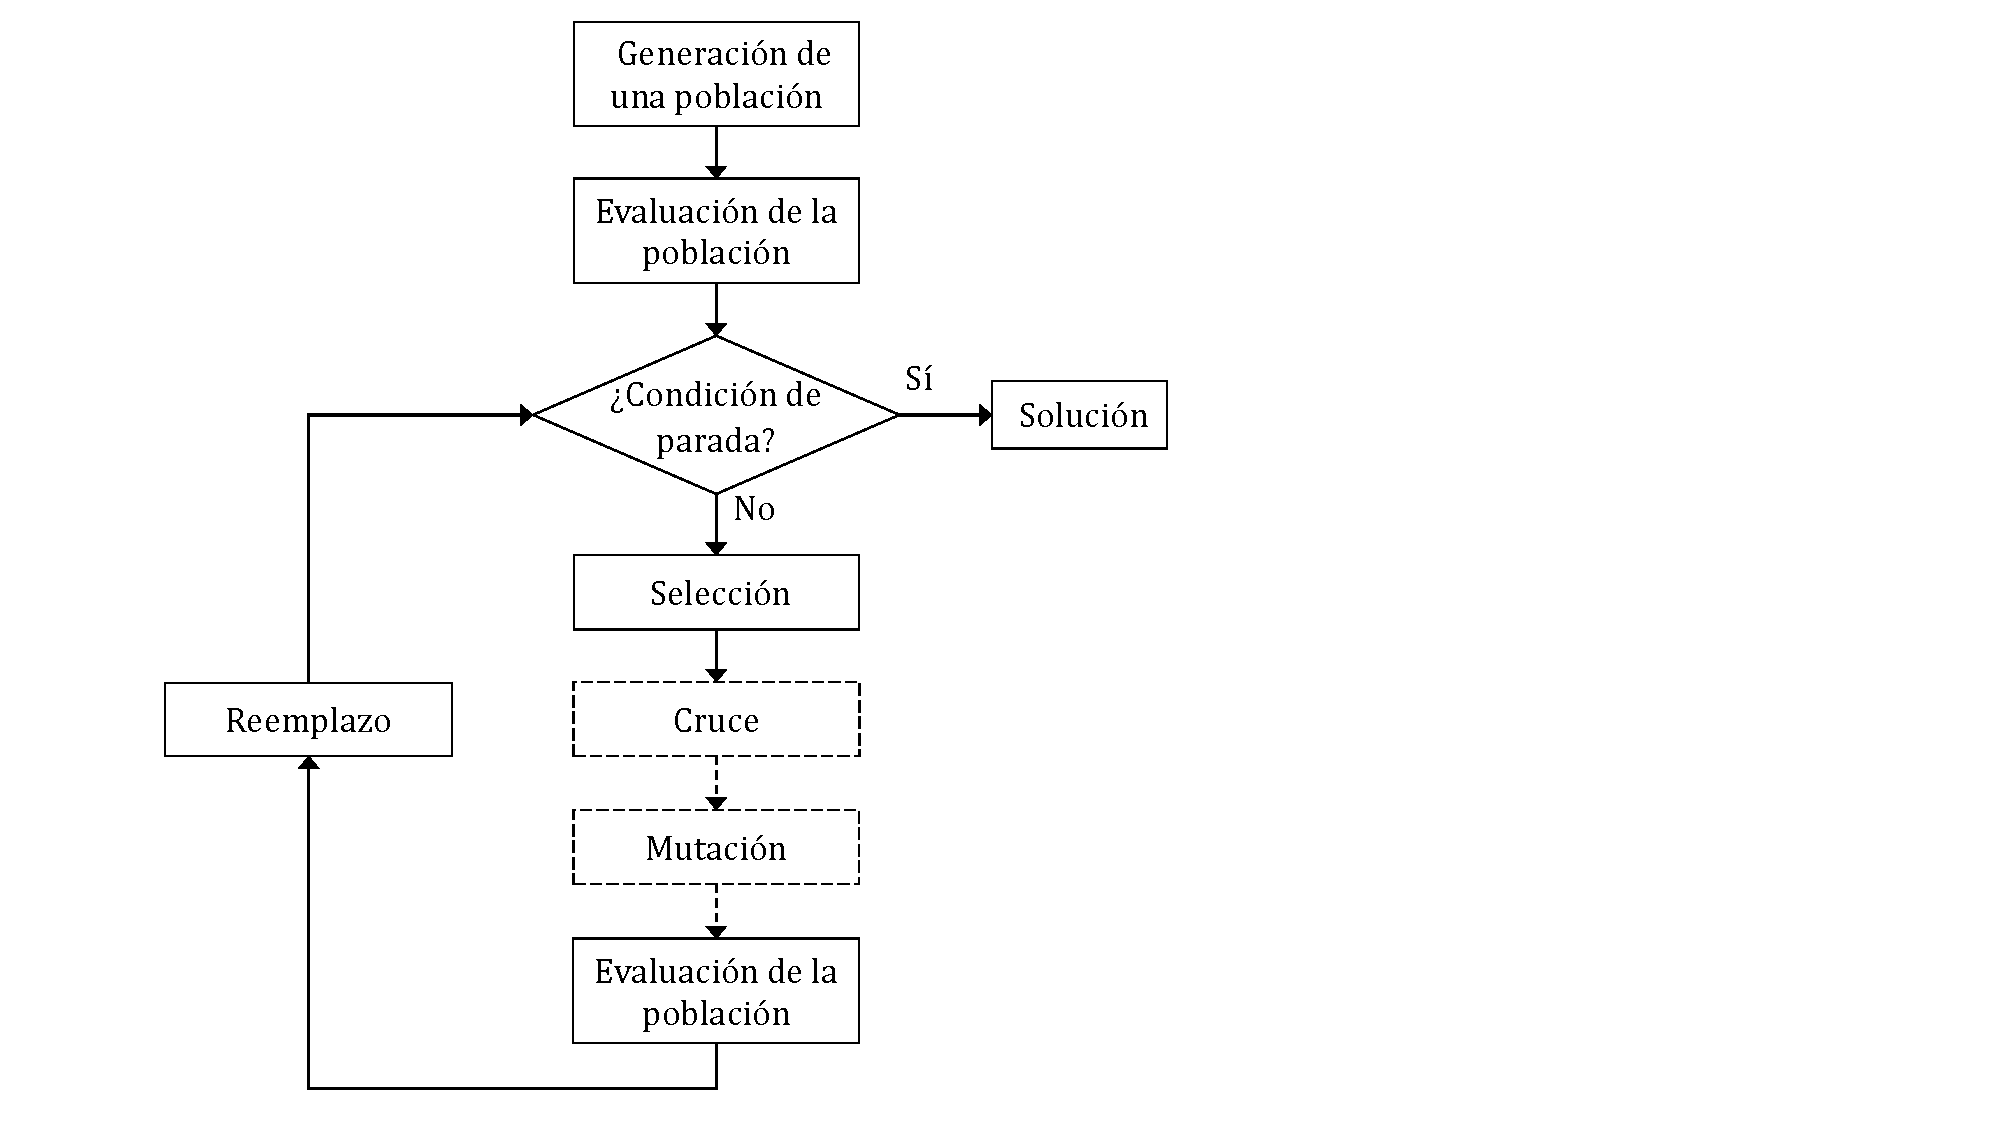
\includegraphics[width = 1\textwidth]{resources/Fig1.pdf}
    \caption{Ciclo Evolutivo que rige el desarrollo de los algoritmos en la Computación Evolutiva.}
    \label{fig:1}
  \end{figure}
  En Fig. \ref{fig:1} se puede apreciar este Ciclo Evolutivo. Todo comienza con una población inicial, que se corresponderá con un conjunto de individuos $Z$ de tamaño $\alpha$ que serán seleccionados del espacio de búsqueda $E$, que es la codificación, completa o no, dependiendo del alfabeto $A$ utilizado en este proceso, del espacio de soluciones $S$. Esta codificación se lleva a cabo mediante una función de codificación $\Omega$. La elección del alfabeto $A$ es fundamental, ya que, dependiendo de su precisión, puede que haya individuos del espacio $S$ que no tengan representación en el espacio $E$, y si es una solución potencialmente buena (incluyendo la óptima), entonces el proceso evolutivo nunca la encontrará. \par
  Tras la conformación de la población inicial (a partir del espacio de búsqueda $E$), se evalúa, por medio de una función de evaluación (\emph{fitness function}), a sus individuos para determinar su grado de adaptación, de tal forma que un valor muy alto implicará que ese individuo tiene un grado mejor de adaptabilidad que otro cuyo valor sea más bajo (y que, por tanto, tendrá más probabilidades de mantenerse en la población inicial). Para este proceso de evaluación, en algunas ocasiones, hará falta decodificar a los individuos, por lo que se aplicará la función de decodificación $\Omega^{-1}$. \par \vfill
  Tras el proceso de generación de la población inicial $Z$, se determina si se cumple la condición de parada (\emph{stop condition}), que es un compendio de condiciones lógicas que detiene el ciclo evolutivo si se cumple, y en caso contrario, continúa. Las condiciones siguen un estricto e inalterable orden que permite el correcto funcionamiento de este proceso.
  \begin{enumerate}
    \item Algún individuo de la población contiene la solución óptima al problema.
    \item La población ha convergido (a una solución óptima o no).
    \item Se ha alcanzado el número máximo de generaciones.
  \end{enumerate} \par
  En el primer caso, la ejecución finaliza devolviendo el individuo óptimo y, por tanto, encontrando la solución. Si la población converge sin haber encontrado antes un individuo óptimo (la población evoluciona después de comprobar la condición de parada, por lo que puede que haya convergido a la optimalidad después de la comprobación previa), entonces finaliza devolviendo cualesquiera de los individuos de la misma. Si no se cumple ninguna de estas dos condiciones, entonces se comprueba si se han superado el número de generaciones máximas determinadas por el usuario. En caso afirmativo, finaliza devolviendo el mejor individuo (no óptimo) de la población. En el caso de que no se cumpla ninguna condición de parada, el algoritmo continúa. \par
  Después, si la población no ha sufrido una evolución en la generación anterior, entonces se aplican los operadores genéticos de selección (\emph{selection}), cruce (\emph{crossover}) y mutación (\emph{mutation}) sobre los individuos. Tras aplicar estos tres operadores, se evalúa la población resultante y se comprueba si se cumple la condición de parada. Si a la población si se le han aplicado estos operadores, entonces se aplica solo el operador genético de reemplazo (\emph{replace}), que generará una nueva población y el proceso se repetirá hasta que se cumpla la condición de parada. \par
  Como se ha mencionado, existen un total de cuatro operadores genéticos que actúan, dependiendo del tipo, sobre la propia población $Z$ o el espacio de búsqueda $E$. Estos operadores se definen como:
  \begin{itemize}
    \item Selección. Es el operador encargado de elegir a los individuos de $Z$ que se cruzarán para generar otros nuevos. La cantidad de individuos seleccionados $\pi$ coincidirá con la cantidad de descendientes producidos. El fundamento radica que en la naturaleza, aquellos individuos mejor adaptados tendrán una probabilidad de reproducción mayor frente aquellos que no lo estén. Por tanto, una implementación tradicional consiste en seleccionar con mayor probabilidad a los mejor adaptados, pero hay otras elitistas que seleccionan solo a los $\pi$ mejor adaptados, desechando a los peores individuos.
    \item Cruce. Los individuos seleccionados por el operador anterior acceden al \emph{mating pool}. Estos individuos reciben el nombre de progenitores (\emph{progenitors}) y que se reproducirán para conformar su descendencia (\emph{offspring}). Normalmente, los progenitores se reproducen por parejas, conformando 2 descendientes. A rasgos del ciclo, este operador es opcional para muchos individuos de la población, ya que no todos son seleccionados. Este operador se aplica sobre los individuos de la población, pero permite generar otros individuos nuevos del espacio $E$ y que no estaban codificados en ningún otro individuo de la población, aumentando la diversidad.
    \item Mutación. Con cierta probabilidad (normalmente entre un 5 y un 10\%), un individuo de la población $Z$ experimenta cambios en su genoma (\emph{genome}). Esto permite aumentar la diversidad de la población al generar otra posible solución potencial (puede ser peor o mejor que el individuo previo a la mutación).
    \item Reemplazo. Este operador selecciona a los $\alpha$ individuos que formarán parte de la siguiente generación, es decir, de la nueva población si no se cumple la condición de parada después de aplicar los tres operadores anteriores. Hay muchas políticas de reemplazo, pero el fin común es producir la mejora gradual de los individuos generación a generación (o lo que es lo mismo, sustituir las peores soluciones con otras mejores).
  \end{itemize} \par
  Se puede apreciar que los operadores resultan indispensables para el desarrollo y mejora de la población y su llegada hacia la solución óptima. En concreto, el cruce es el máximo responsable del proceso evolutivo, ya que es el encargado de generar nueva descendencia, tratando de seleccionar los mejores genes de cada progenitor. \par
  Según los operadores que se seleccionen o implementen, la técnica evolutiva realizará labores de exploración (\emph{exploration}) o de explotación (\emph{exploitation}). La exploración consiste en muestrear regiones desconocidas en el espacio de búsqueda $E$ donde pueden encontrarse las soluciones óptimas. La explotación trata de mejorar al individuo más destacado, acortando la búsqueda de la solución óptima en una búsqueda local. Por tanto, estos operadores (y en especial el operador de cruce) se deben comportar de forma explotativa en las primeras generaciones, ya que hay una gran diversidad y de otra forma se produciría una convergencia muy lenta. Sin embargo, a medida que la población va convergiendo hacia una solución, es necesario que los operadores exploren, es decir, escapen hacia otras regiones de búsqueda. \par
  La mayor parte de las heurísticas que forman parte de la Computación Evolutiva siguen el patrón descrito, salvo aquellas que, debido al problema que abordan, tienen una estructura que difiere al resto.
  
  \section*{\Large 2.3. Programación Genética}
  La Programación Genética (Cramer, 1985; Koza, 1988) es una heurística de la familia de la Computación Evolutiva y que permite resolver problemas de búsqueda y optimización cuya solución es un programa informático. La Programación Genética es una extensión de los Algoritmos Genéticos (Holland, 1967) pero donde el espacio de soluciones $S$ está compuesto por programas informáticos.
    \subsection*{\large 2.3.1. Codificación y representación de los individuos}
    Los individuos en la Programación Genética se representan mediante árboles, conformados por operadores (\emph{operators}) y operandos (\emph{operands}). Los operadores, que son los nodos intermedios y el nodo raíz, representan funciones, mientras que los operandos son los nodos hoja. Esta representación permite la construcción de expresiones matemáticas que son fáciles de evolucionar y de evaluar.
    \begin{figure}[H]
      \centering
      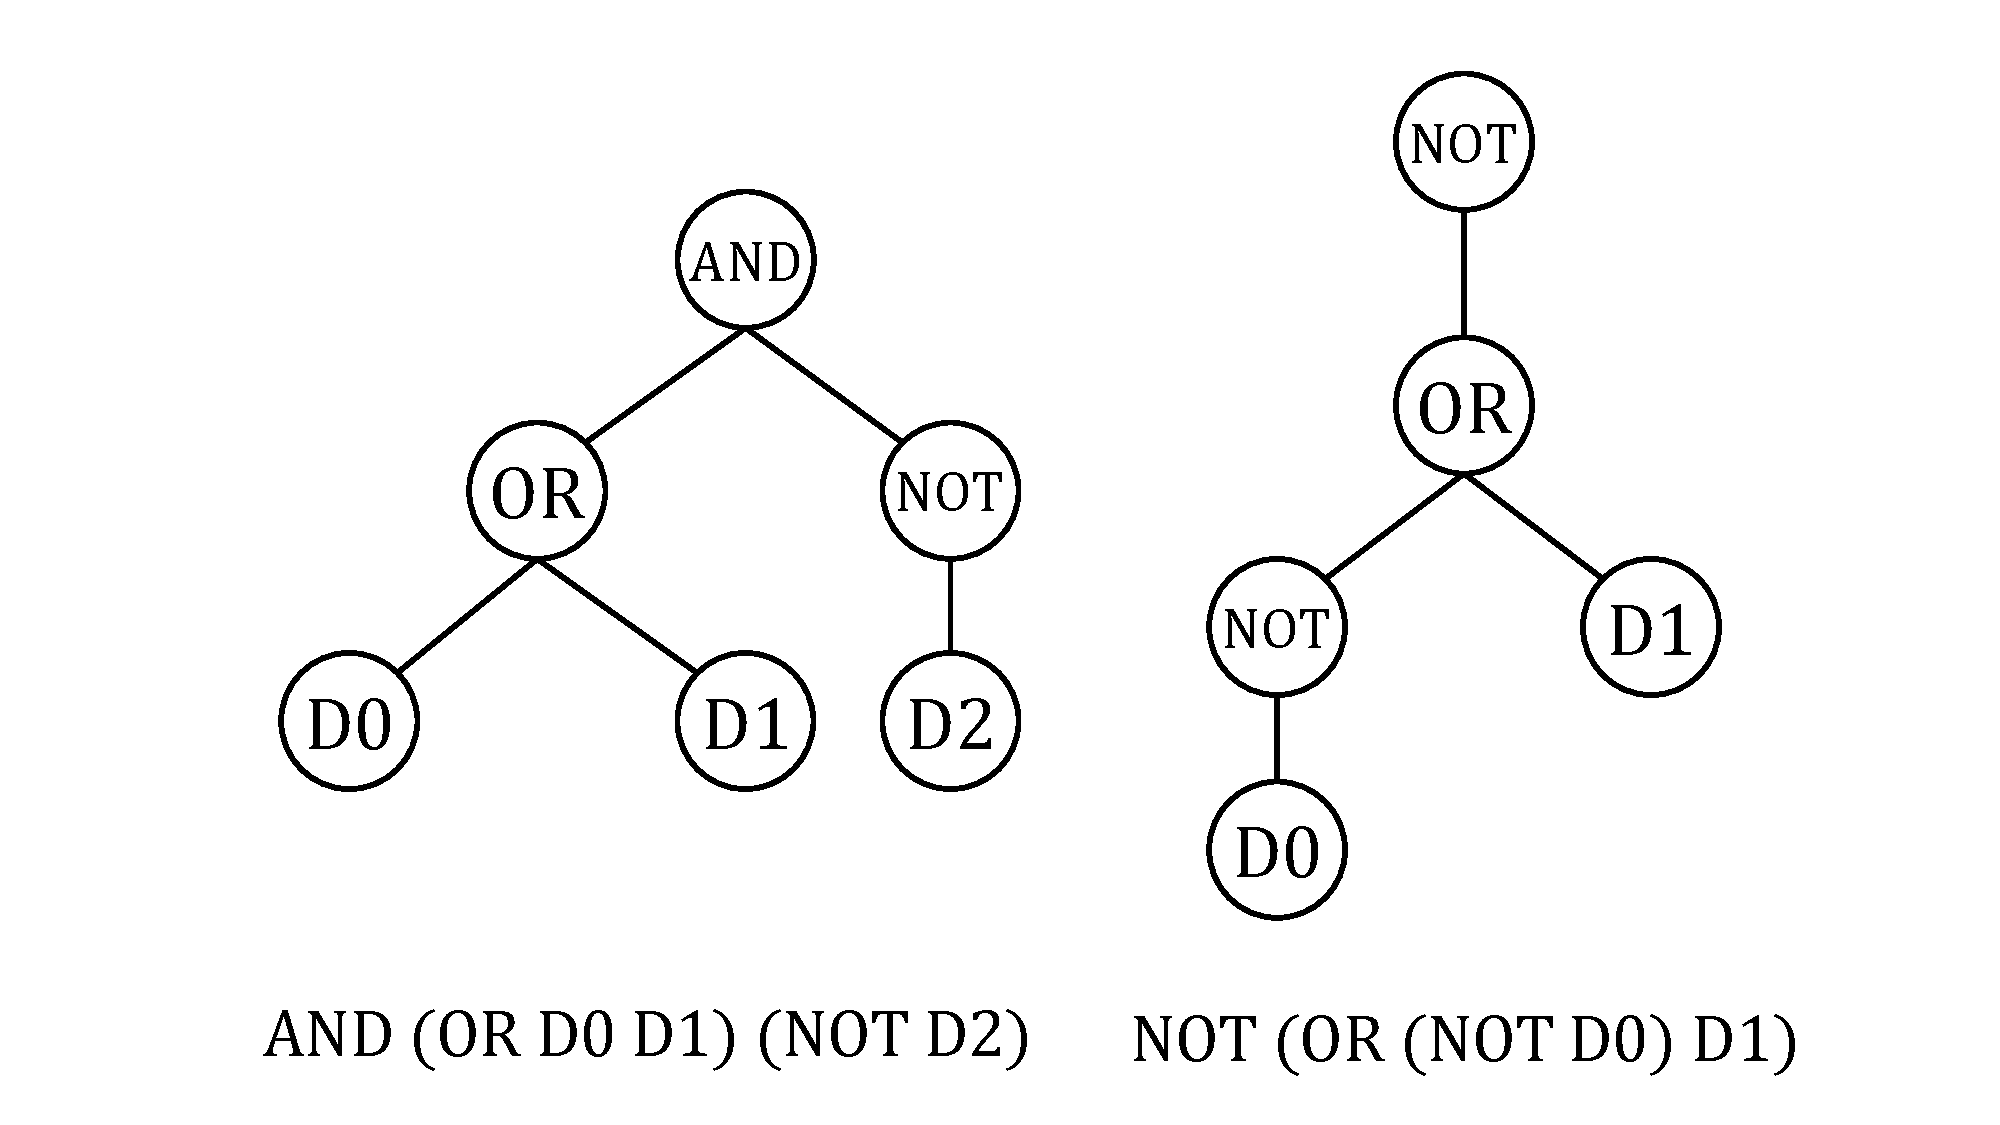
\includegraphics[width = 0.7\textwidth]{resources/Fig2.pdf}
      \caption{Individuos de un programa genético codificados en forma de árbol y su correspondiente decodificación.}
      \label{fig:2}
    \end{figure} \par
    La creación de los individuos debe cumplir dos propiedades. La primera de ellas se refiere a la propiedad del cierre (\emph{closure property}), que evita la creación de individuos sintácticamente inválidos estableciendo que la salida de una función debe poder servir de entrada para otra. La segunda propiedad es la explosión de código (\emph{code bloat}) (Tackett, 1995), que recoge el crecimiento desmesurado del código sin mejora de la adaptación, y, por lo tanto, debería evitarse en la medida de lo posible, ya que propicia el aparecimiento de intrones (\emph{introns}), que son fragmentos de código totalmente inútiles ya que no favorecen la adaptación y que se traduce en una convergencia lenta y una demora en la evaluación de los individuos. Además, el alfabeto $A$ con el que se vayan a codificar los elementos del espacio de soluciones $S$ estará formado por operadores y operandos, buscando en la medida de lo posible la biyección. Para la codificación, se lee de arriba a abajo y de izquierda a derecha.
  
    \subsection*{\large 2.3.2. Operadores}
    La Programación Genética cuenta con cuatro operadores: selección, cruce, mutación y reemplazo. Aquellos que actúan sobre la población y no sobre el espacio de búsqueda son el de selección y el de reemplazo, por lo que funcionan de forma análoga a como hacen en otras heurísticas como en los Algoritmos Genéticos o en la Evolución Gramatical, por lo que solo se explicará el operador de cruce y el de mutación.
    
      \subsubsection*{\normalsize 2.3.2.1. Cruce}
      El operador de cruce se aplica sobre los individuos que han sido seleccionados y que se encuentran en el mating pool. Al tratarse de árboles, es necesario que los operadores que se utilizan en el proceso evolutivo aseguren que se cumple la propiedad del cierre y la de la explosión de código. \par
      
        \subsubsection*{\vspace{-0.5cm}{\normalsize Operador de Koza}}
        \vspace{-0.5cm}
        El operador de cruce de Koza (Koza, 1992) selecciona un nodo de cada padre de forma aleatoria y se intercambian los subárboles. Aparentemente, en la Programación Genética tradicional este operador funciona sin errores ya que genera individuos sintácticamente correctos, cumpliéndose la propiedad del cierre. Sin embargo, como en el ejemplo mostrado en Fig. \ref{fig:3}, se corre el riesgo de que se produzcan intrones como consecuencia de la explosión de código, ya que no cuenta con un mecanismo de control de profundidad.
        \begin{figure}[H]
          \centering
          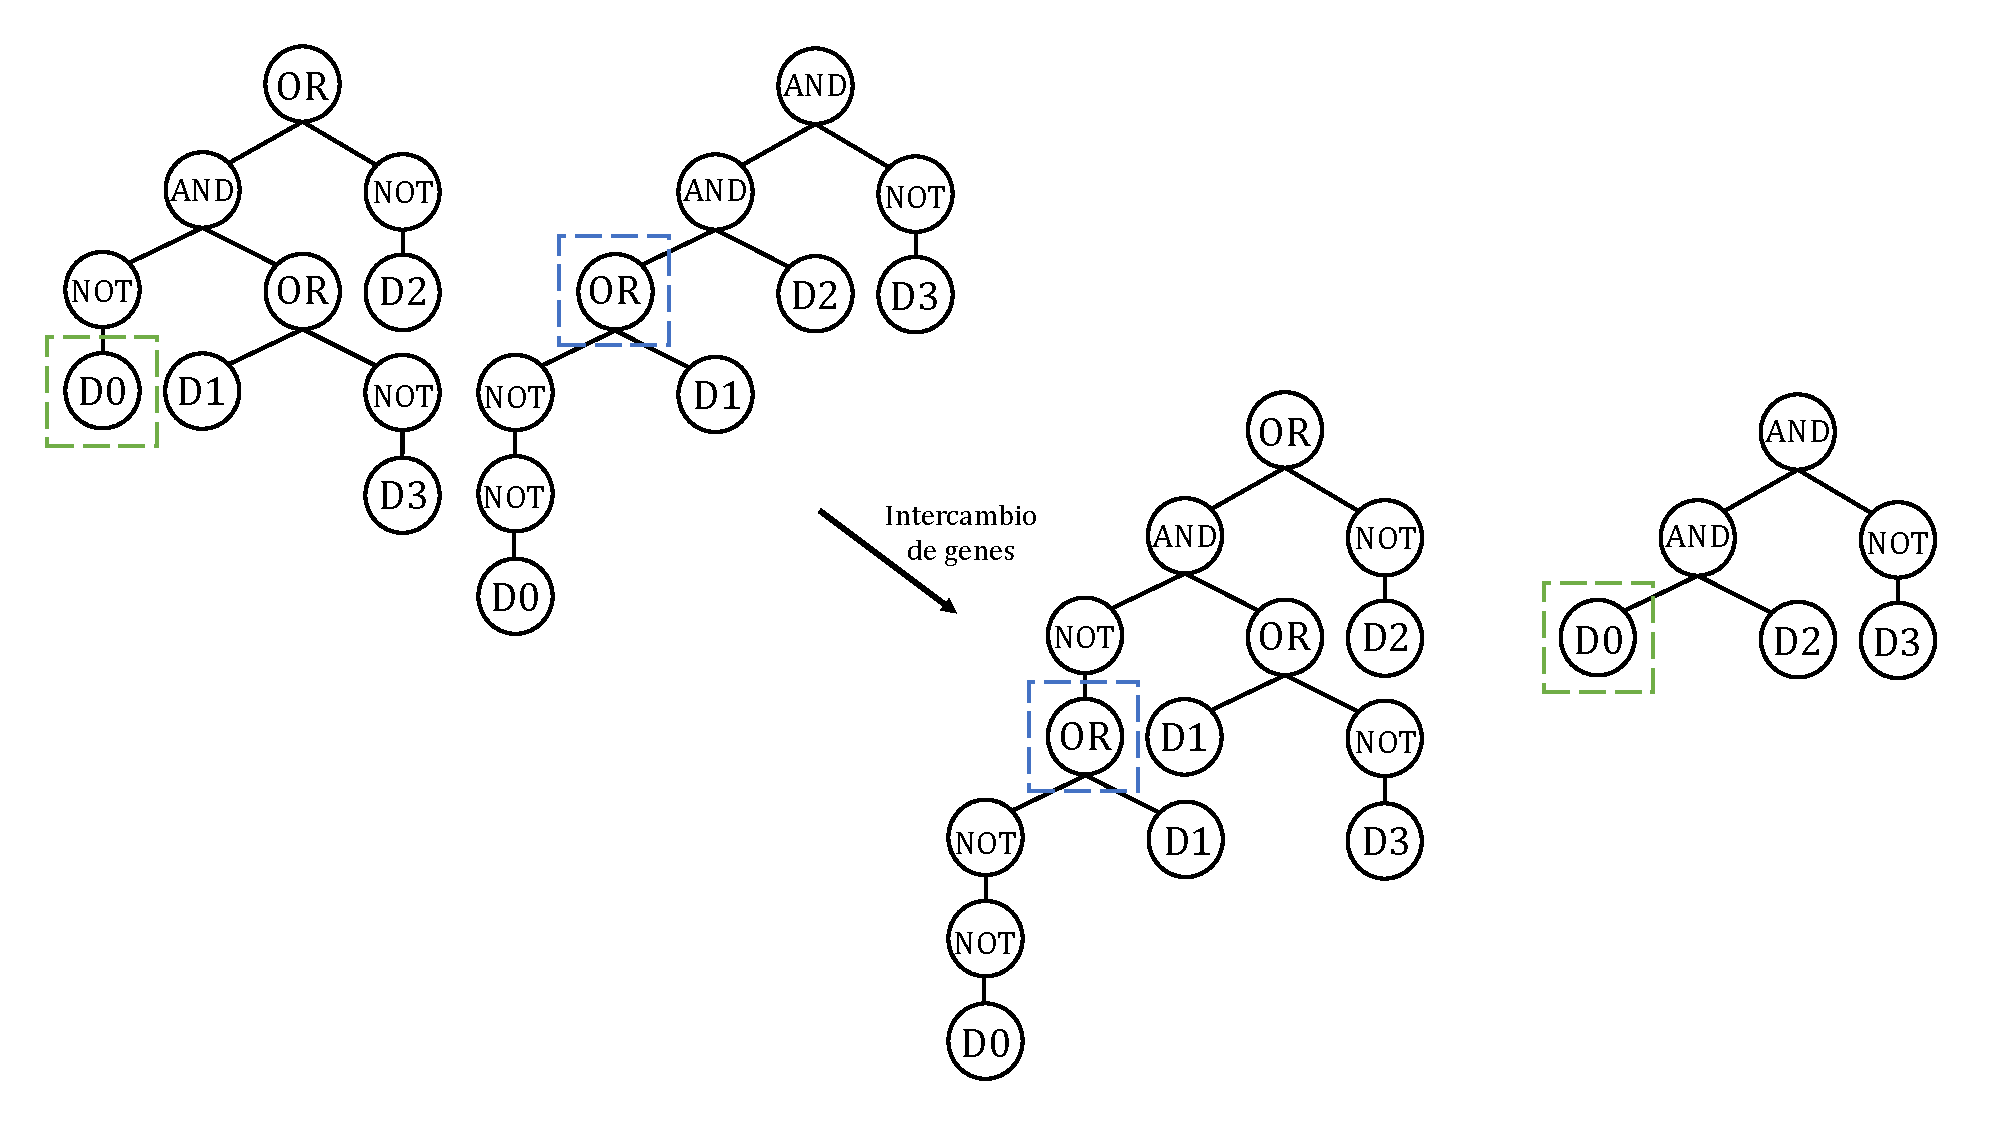
\includegraphics[width = 1\textwidth]{resources/Fig3.pdf}
          \caption{Ejemplo de aplicación del operador de cruce de Koza.}
          \label{fig:3}
        \end{figure} \par
        Sin embargo, en la Programación Genética Guiada por Gramáticas, este operador no es útil ya que genera individuos que no respetan las reglas de derivación de la gramática utilizada.
        
        \subsubsection*{\vspace{-0.5cm}{\normalsize Operador basado en un punto}}
        \vspace{-0.5cm}
        El operador de cruce basado en un punto (Poli and Langdon, 1997a, 1997b, 1998) de la Programación Genética se inspira en el igualmente llamado de los Algoritmos Genéticos (Goldberg, 1989). Este operador selecciona el nodo de cruce después de un proceso de alineamiento (\emph{alignment}) entre los padres, donde se seleccionan los nodos potenciales para realizar el intercambio.
        \begin{figure}[H]
          \centering
          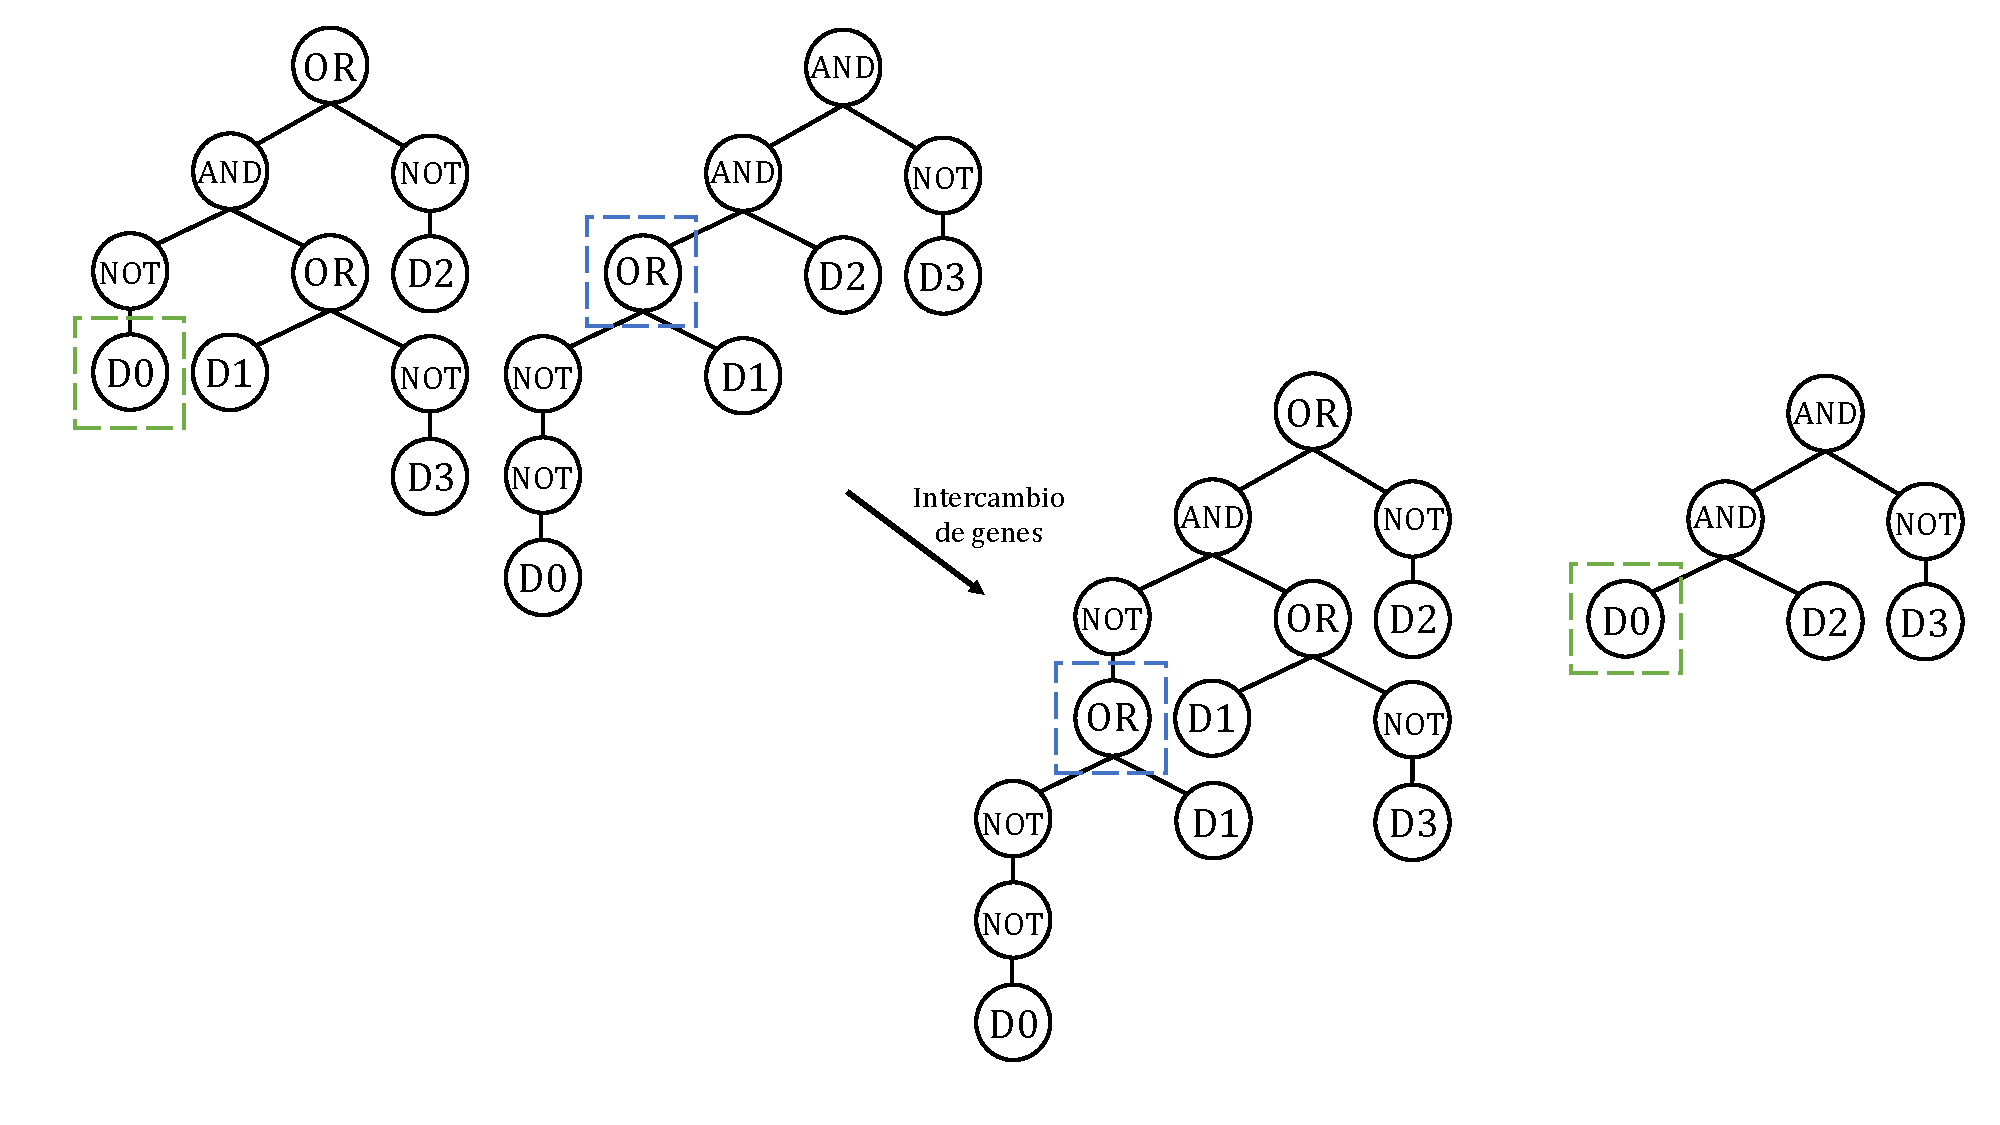
\includegraphics[width = 1\textwidth]{resources/Fig4.pdf}
          \caption{Ejemplo de aplicación del operador de cruce basado en un punto.}
          \label{fig:4}
        \end{figure} \par
        Este operador selecciona un nodo de forma aleatoria de entre los coincidentes entre los dos padres. El problema que tiene este operador es que si la estructura de los padres es totalmente distinta, los descendientes coincidirán con los padres y su genoma será el mismo.
        
      \subsubsection*{\normalsize 2.3.2.2. Mutación}
      El operador de mutación se aplica con una muy baja probabilidad (de entre el 5 y el 10\%) a un individuo en cada generación. Debido a la baja probabilidad, puede que haya ejecuciones completas en las que no se haya dado ningún caso de mutación. De hecho, hay programas genéticos que no utilizan este operador. Al no existir una gramática que contenga reglas de derivación, este operador selecciona un nodo de forma aleatoria en el individuo seleccionado, y a continuación, genera un subárbol a partir de ese nodo seleccionado de forma análoga a como se inicializan las poblaciones en esta heurística, reparando al individuo resultante si fuera necesario.
  
    \subsection*{\large 2.3.3. Generación de la población inicial}
    El programa genético debe partir de una población de individuos inicial $Z$, que es un subconjunto del espacio de búsqueda $E$. La metodología de creación de individuos en Programación Genética es aleatoria, ya que no existen gramáticas que regulen su formación (como sucede por el contrario en la Programación Genética Guiada por Gramáticas). \par
    Al generar individuos de forma aleatoria, hay una gran probabilidad de que no se cumplan las propiedades que gobiernan la Programación Genética: la propiedad del cierre y la de la explosión de código. Por tanto, es necesario un proceso de reparación de individuos. Normalmente, se basan en la sustitución de nodos mal colocados por otros correctos de forma aleatoria, como en Fig. \ref{fig:5}. \par
    \begin{figure}[H]
      \centering
      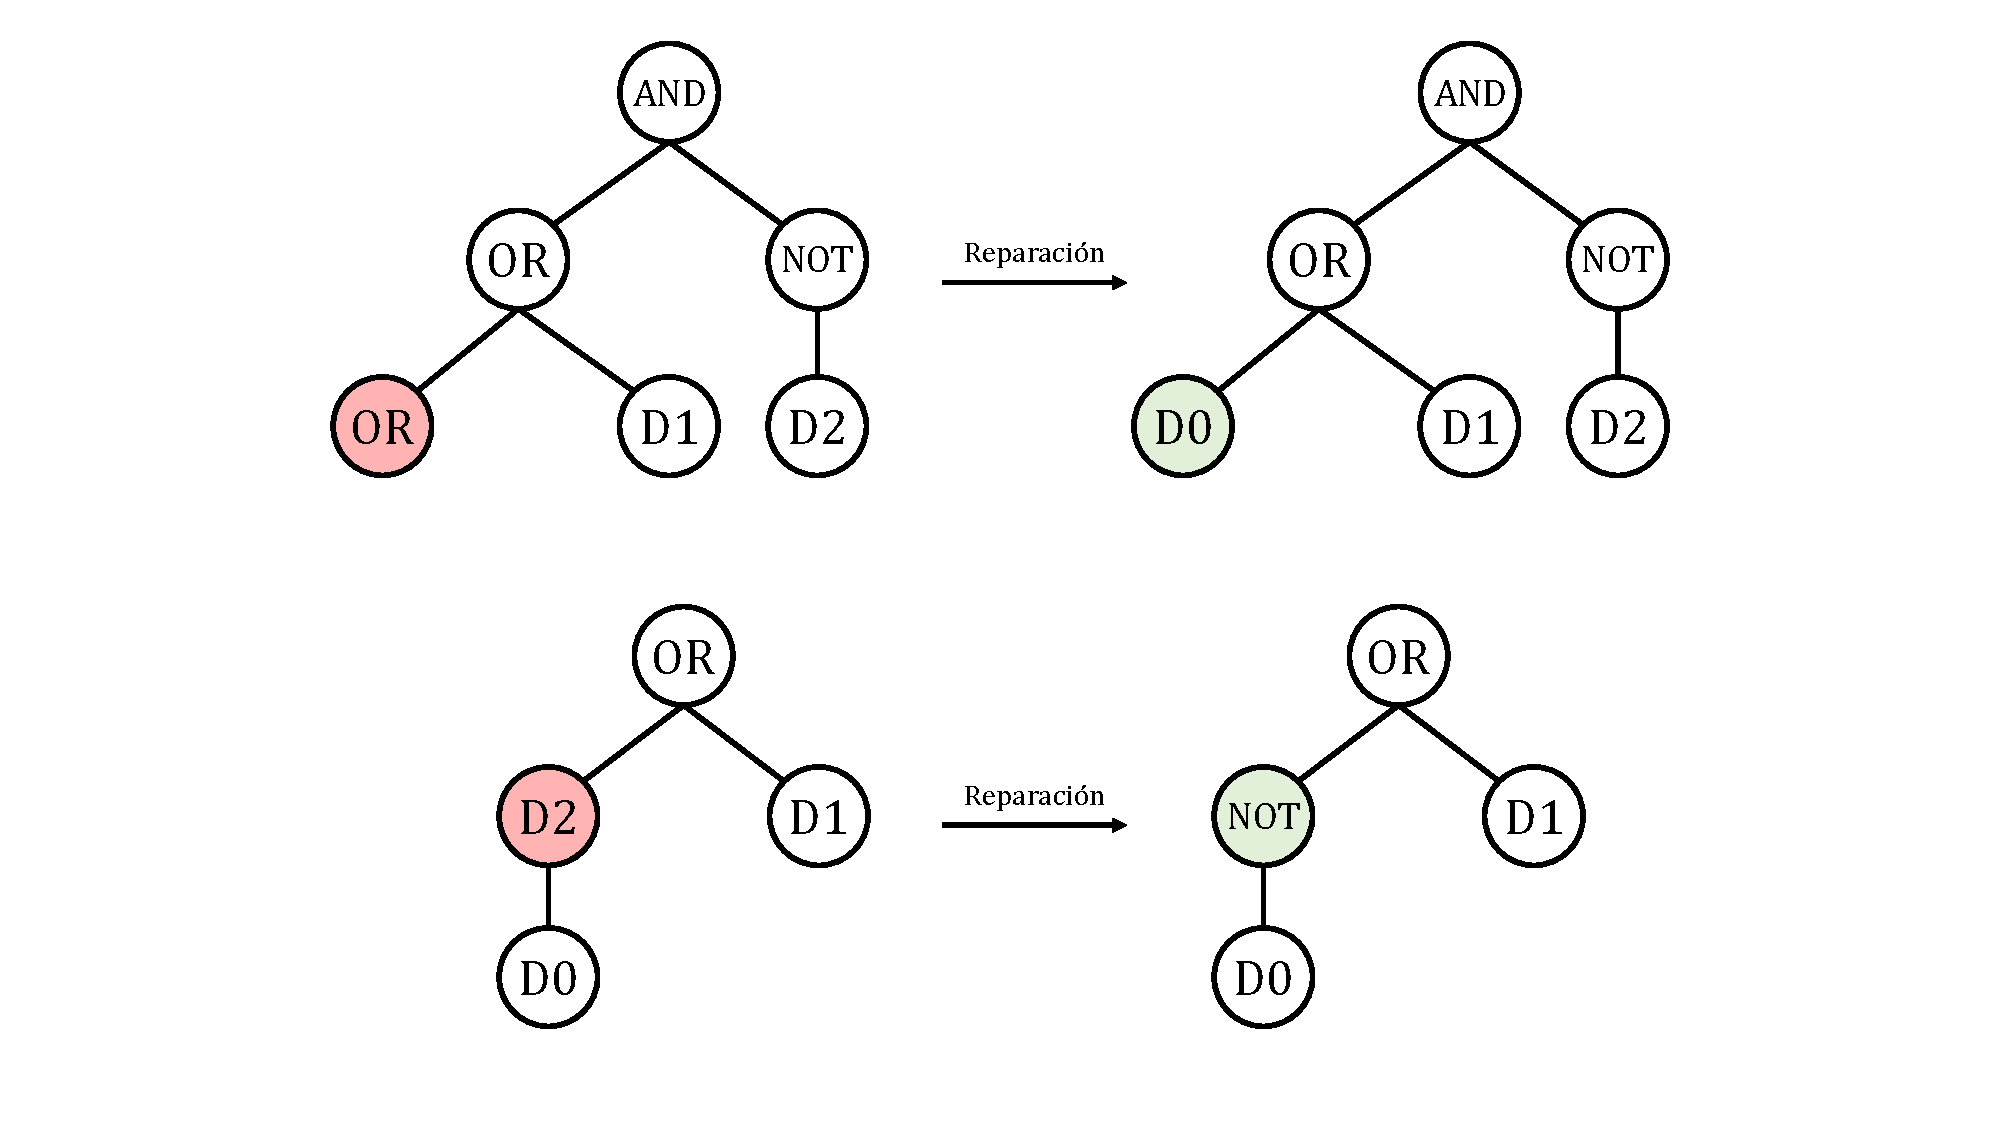
\includegraphics[width = 1\textwidth]{resources/Fig5.pdf}
      \caption{Ejemplo de aplicación de la función de reparación de individuos inválidos.}
      \label{fig:5}
    \end{figure} \par
    Este proceso de reparación muchas veces es más tardío que la generación de un nuevo individuo, por lo que en la práctica los individuos inválidos se descartan y se sustituyen por otros, que si son nuevamente inválidos se descartan, repitiendo ese proceso hasta que se alcanza una población $Z$ de tamaño $\alpha$.

  \section*{\Large 2.4. Programación Genética Guiada por Gramáticas}
  La Programación Genética Guiada por Gramáticas (Whigham, 1995) surge por las dificultades encontradas en el desarrollo de los programas genéticos en relación con sus dos propiedades: la propiedad del cierre y la explosión de código. En concreto, la aleatoriedad en la creación de individuos resulta una carga cuando los problemas son grandes y la cantidad de símbolos es elevada, pues hay más probabilidades de generar un individuo inválido (Vanneschi et al., 2010). Además, la función de reparación o la sustitución de individuos inválidos por otros bien formados es una pérdida de tiempo y aumenta la complejidad computacional en buena medida. \par
  La Programación Genética Guiada por Gramáticas acaba con los problemas de la creación de individuos inválidos gracias a la utilización de Gramáticas Libres de Contexto (\emph{context-free grammars}) (Chomsky, 1959), que permiten que la solución que codifican los individuos forme parte del espacio de búsqueda $E$, y por tanto, se cumpla el propiedad del cierre aunque estos individuos sean generados de forma aleatoria.
  
    \subsection*{\large 2.4.1. Gramáticas Libres de Contexto}
    Una Gramática Libre de Contexto $G$ está definida por una 4-tupla (Hopcroft and Ullman, 1979) de la forma: 
    \begin{align}
    G = (\Sigma_{N}, \Sigma_{T}, S, P), \label{eq:1}\tag{1}
    \end{align}
    donde $\Sigma_{N}$ se corresponde con el conjunto de símbolos no terminales (variables), $\Sigma_{T}$ con el conjunto de símbolos terminales (constantes), $S$ es el axioma o símbolo principal, del que derivarán las reglas que conformen al individuo y $P$ es el conjunto de reglas de producción. \par
    Una regla de producción (\emph{production rule}) de $P$ tienen la forma $\alpha \rightarrow \beta$, donde $\alpha$ es un símbolo no terminal con $\alpha \in \Sigma_{N}$ y $\beta$ es una cadena de variables y/o terminales con $\beta \in (\Sigma_{N} \cup \Sigma_{T})$. \par
    Una derivación (\emph{derivation}) de la gramática $G$ se puede entender como una regla $R$ perteneciente a $S$ tal que $\alpha \rightarrow \beta$. Esta derivación tiene asociada una palabra (\emph{word}), que se corresponde con la decodificación del individuo en el espacio $S$. \par
    La Programación Genética Guiada por Gramáticas favorece la convergencia de los individuos al eliminar el problema del cierre. También, asegura que los individuos generados son siempre válidos y limita formalmente a los individuos que siempre tendrán una sintaxis basada en las reglas de producción acotadas. Sin embargo, para reglas de producción concretas se pueden producir ciclos, luego la profundidad de un individuo no se puede controlar con estas gramáticas. \par
    Otro problema de estas gramáticas es que puede haber redundancia (\emph{redundancy}), es decir, puede generar dos individuos distintos estructuralmente pero que deriven la misma palabra. Por ejemplo, la siguiente gramática es redundante: \\
    \begin{align*}
    G &= (\Sigma_{N}, \Sigma_{T}, S, P) \label{eq:2}\tag{2} \\
    \Sigma_{N} &= \{S, E, F, N\} \\
    \Sigma_{T} &= \{0, 1, 2, 3, 4, 5, 6, 7, 8, 9, +, -, =\} \\
    P &= \{ \\
    &S ::= E = N \\
    &E ::= E + E | E - E | F + E | F - E | N \\
    &F ::= N \\
    &N ::= 0 | 1 | 2 | 3 | 4 | 5 | 6 | 7 | 8 | 9 \\
    \}
    \end{align*} \par
    Con esta gramática, se han representado dos individuos que reflejan esta condición en Fig. \ref{fig:6}. Se puede comprobar que los símbolos terminales $F$ y $E$ son equivalentes, ya que derivan reglas idénticas. \par
    \begin{figure}[H]
      \centering
      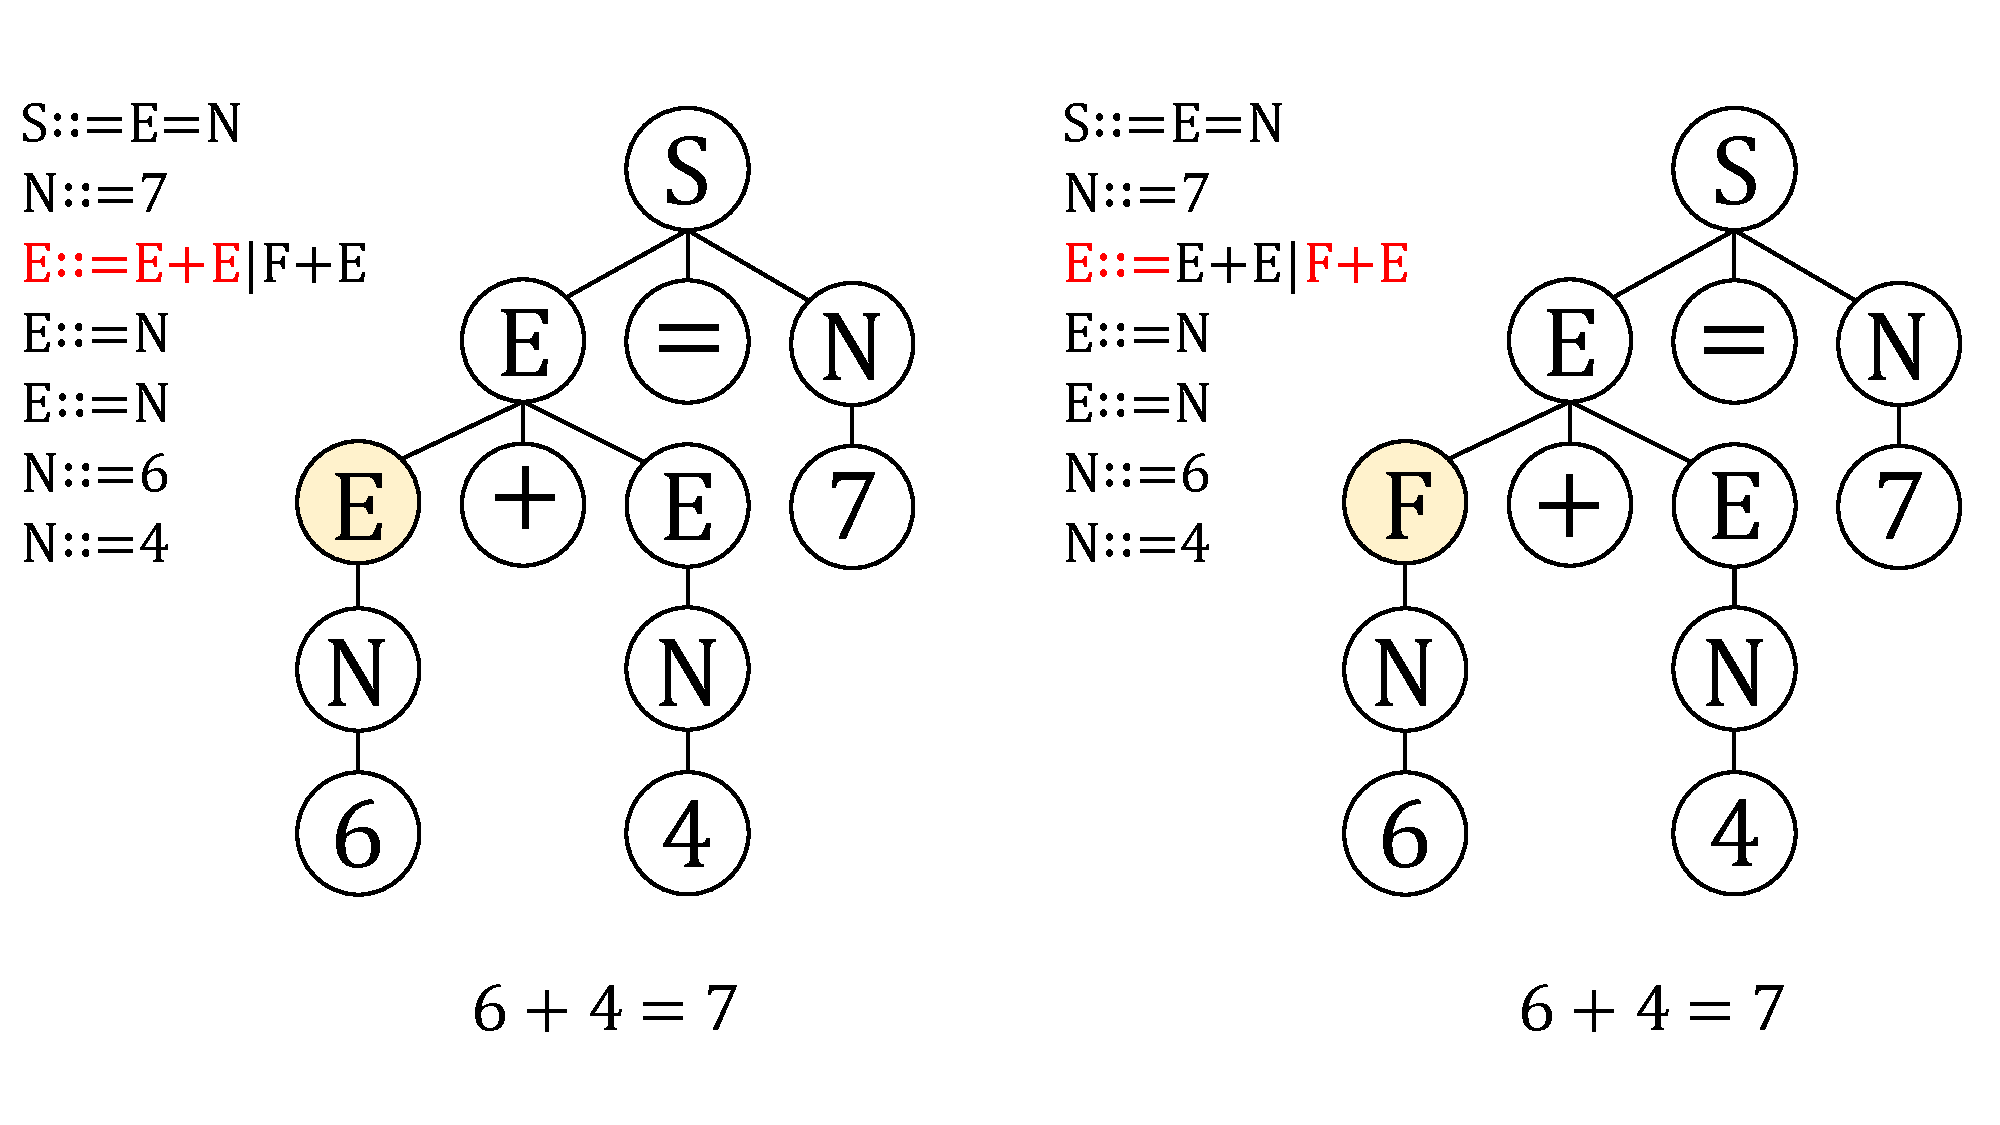
\includegraphics[width = 0.8\textwidth]{resources/Fig6.pdf}
      \caption{Individuos conformados por una gramática redundante.}
      \label{fig:6}
    \end{figure} \par
    Una gramática sin redundancia es una gramática depurada. Algunas veces, la redundancia es útil, ya que, por ejemplo, la solución óptima puede ser alcanzada de forma más fácil si está codificada varias veces. Como inconveniente, se produce una convergencia tardía.
    
    \subsection*{\large 2.4.2. Codificación y representación de los individuos}
    Como sucedía con la Programación Genética, los individuos se representan en forma de árbol. Estos árboles son creados empleando una Gramática Libre de Contexto. La codificación de estos individuos, al contrario de lo que sucedía con la Programación Genética, se obtiene leyendo los nodos terminales de izquierda a derecha, sin incluir los nodos interiores. \par
    La Programación Genética Guiada por Gramáticas cumple con la propiedad del cierre gracias a las gramáticas, asegurando la creación de individuos sintácticamente válidos. Sin embargo, la explosión de código se ve en entredicho o no, dependiendo de si la gramática tiende a formar ciclos. \par
    Una gramática formará ciclos cuando las reglas de producción se llamen a sí mismas en su consecuente. Por ejemplo, la gramática mostrada en Eq. \ref{eq:2} es recursiva, ya que tres de las cuatro reglas del nodo no terminal $E$ se llaman a sí mismas. En tal caso, dependiendo del algoritmo de generación de individuos que se utilice, se producirán o no intrones, retrasando la convergencia. Sin embargo, la recursión que puede determinar la regla $E ::= E + E$ no tiene el mismo grado que la regla $E ::= F + E$, ya que en la primera existe una doble recursión.
    
    \subsection*{\large 2.4.3. Operadores}
    Los operadores de la Programación Genética de cruce y mutación son también útiles en la Programación Genética Guiada por Gramáticas, al igual que los operadores comunes de selección y de reemplazo. Con la adición de las gramáticas, han surgido varias implementaciones nuevas sobre el operador de cruce. Sin embargo, el operador de mutación sigue coincidiendo con el algoritmo de generación de individuos seleccinado.
    
      \subsubsection*{\normalsize 2.4.3.1. Cruce}
      Si bien los operadores de cruce de la Programación Genética pueden utilizarse en la Programación Genética Guiada por Gramáticas, los individuos generados con ellos serán inválidos y no cumplirán con la propiedad de cierre. El ejemplo más evidente se hace palpable con el operador de cruce de Koza, que genera puntos de cruce de forma aleatoria y que no tiene en cuenta las reglas de producción, tal y como se muestra en Fig. \ref{fig:7} con la gramática mostrada en Eq. \ref{eq:2}. \par
      \begin{figure}[H]
        \centering
        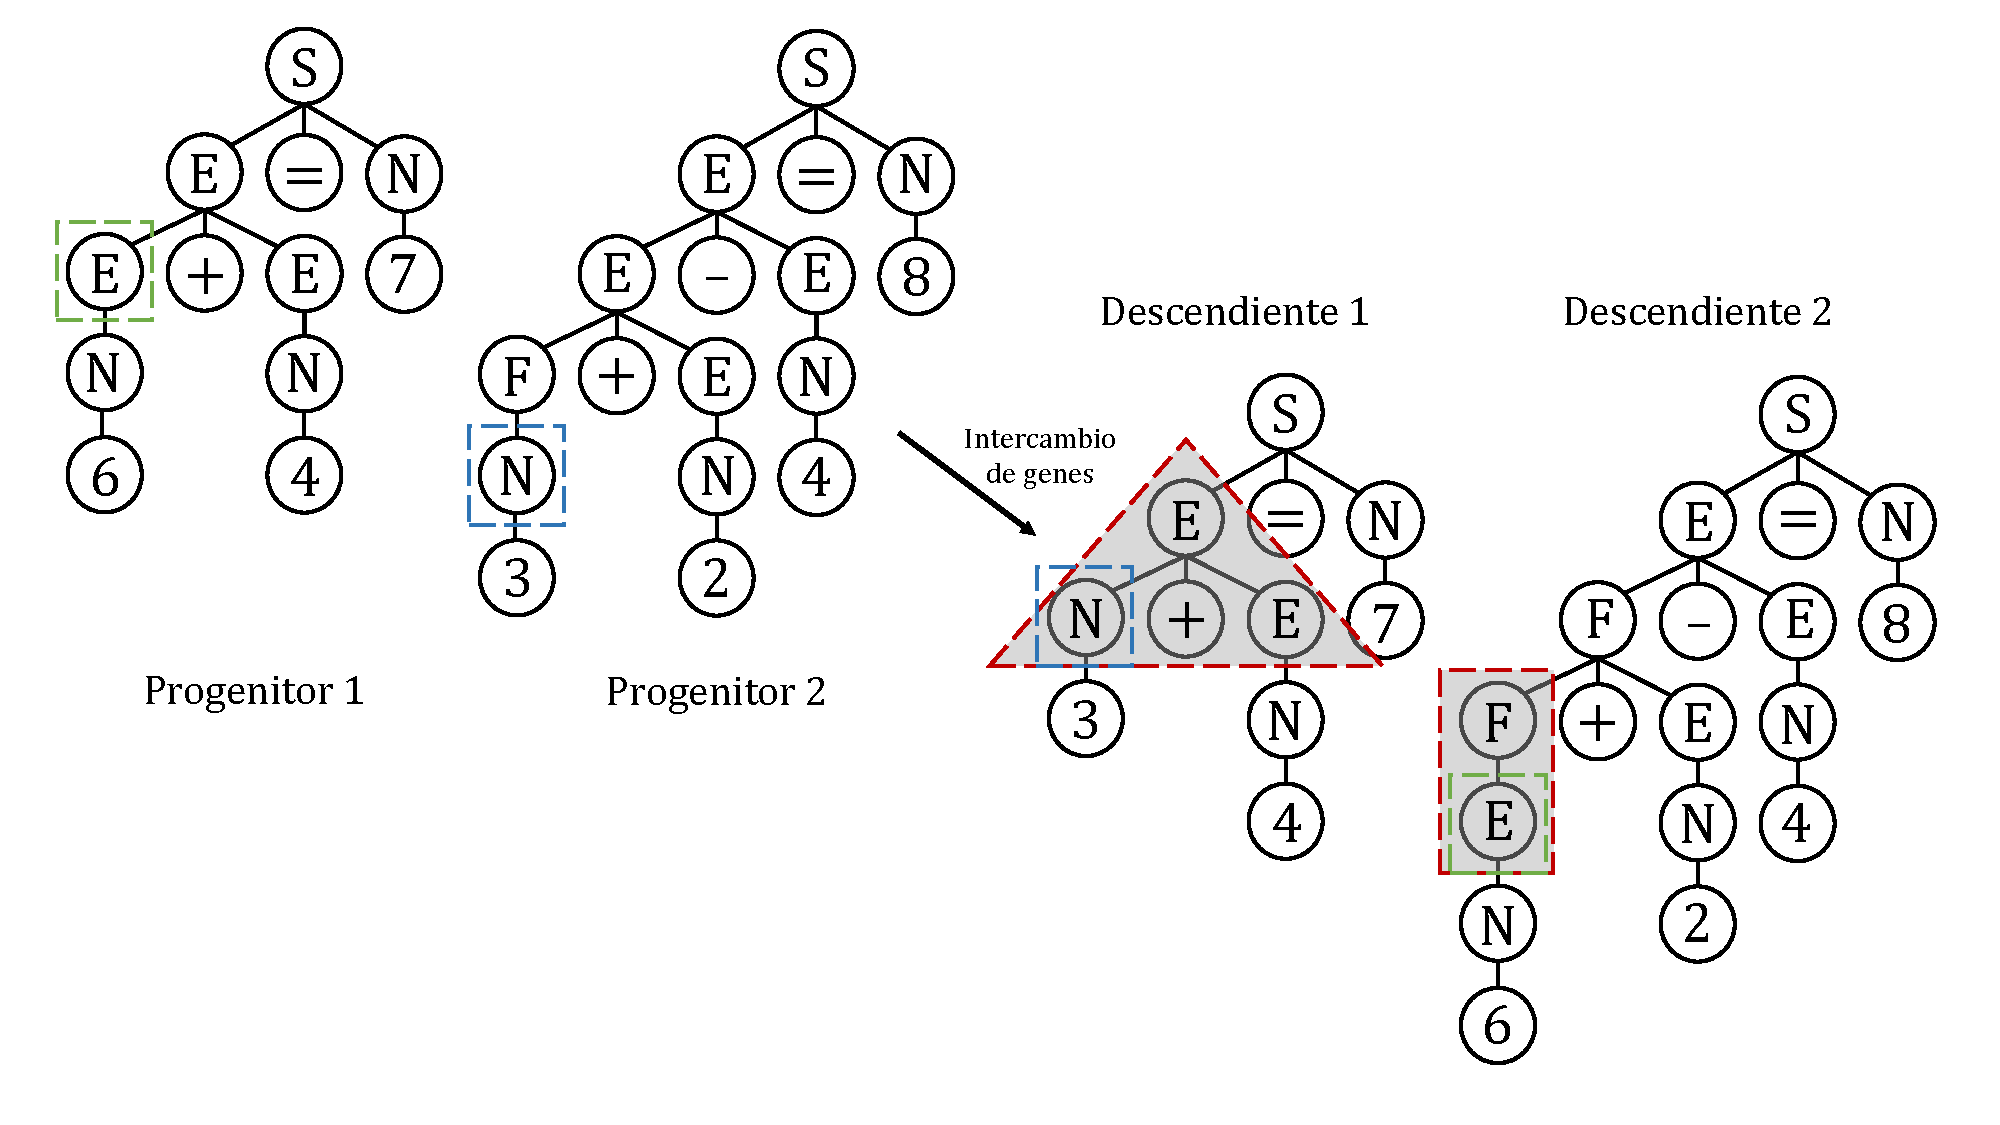
\includegraphics[width = 1\textwidth]{resources/Fig7.pdf}
        \caption{Errores (en rojo) producidos en el cruce de dos individuos generados con gramáticas al aplicar el operador de Koza.}
        \label{fig:7}
      \end{figure} \par
      
        \subsubsection*{\vspace{-0.5cm}{\normalsize Operador de cruce preservador del contexto}}
        \vspace{-0.5cm}
        El operador de cruce preservador del contexto (\emph{context preserving crossover}) (D'haeseleer, 1994) restringe el cruce sólo entre subárboles que tienen localizaciones similares. Estas localizaciones vienen dadas por las coordenadas (\emph{coordinates}), reduciendo el exceso de exploración del operador de Koza. Estas coordenadas se definen como el camino entre la raíz y el nodo elegido. Este cruce sólo selecciona un nodo aleatorio: el del primer progenitor. A continuación, extrae las coordenadas de ese nodo aleatorio y las busca en el segundo progenitor. Si esas coordenadas existen en el segundo progenitor, entonces cruza los árboles. En caso contrario, selecciona otro nodo aleatorio del primer padre, realizando ese proceso repetidamente hasta que se puede efectuar el cruce. En Fig. \ref{fig:8} se puede observar el funcionamiento de este cruce. \par
        \begin{figure}[H]
          \centering
          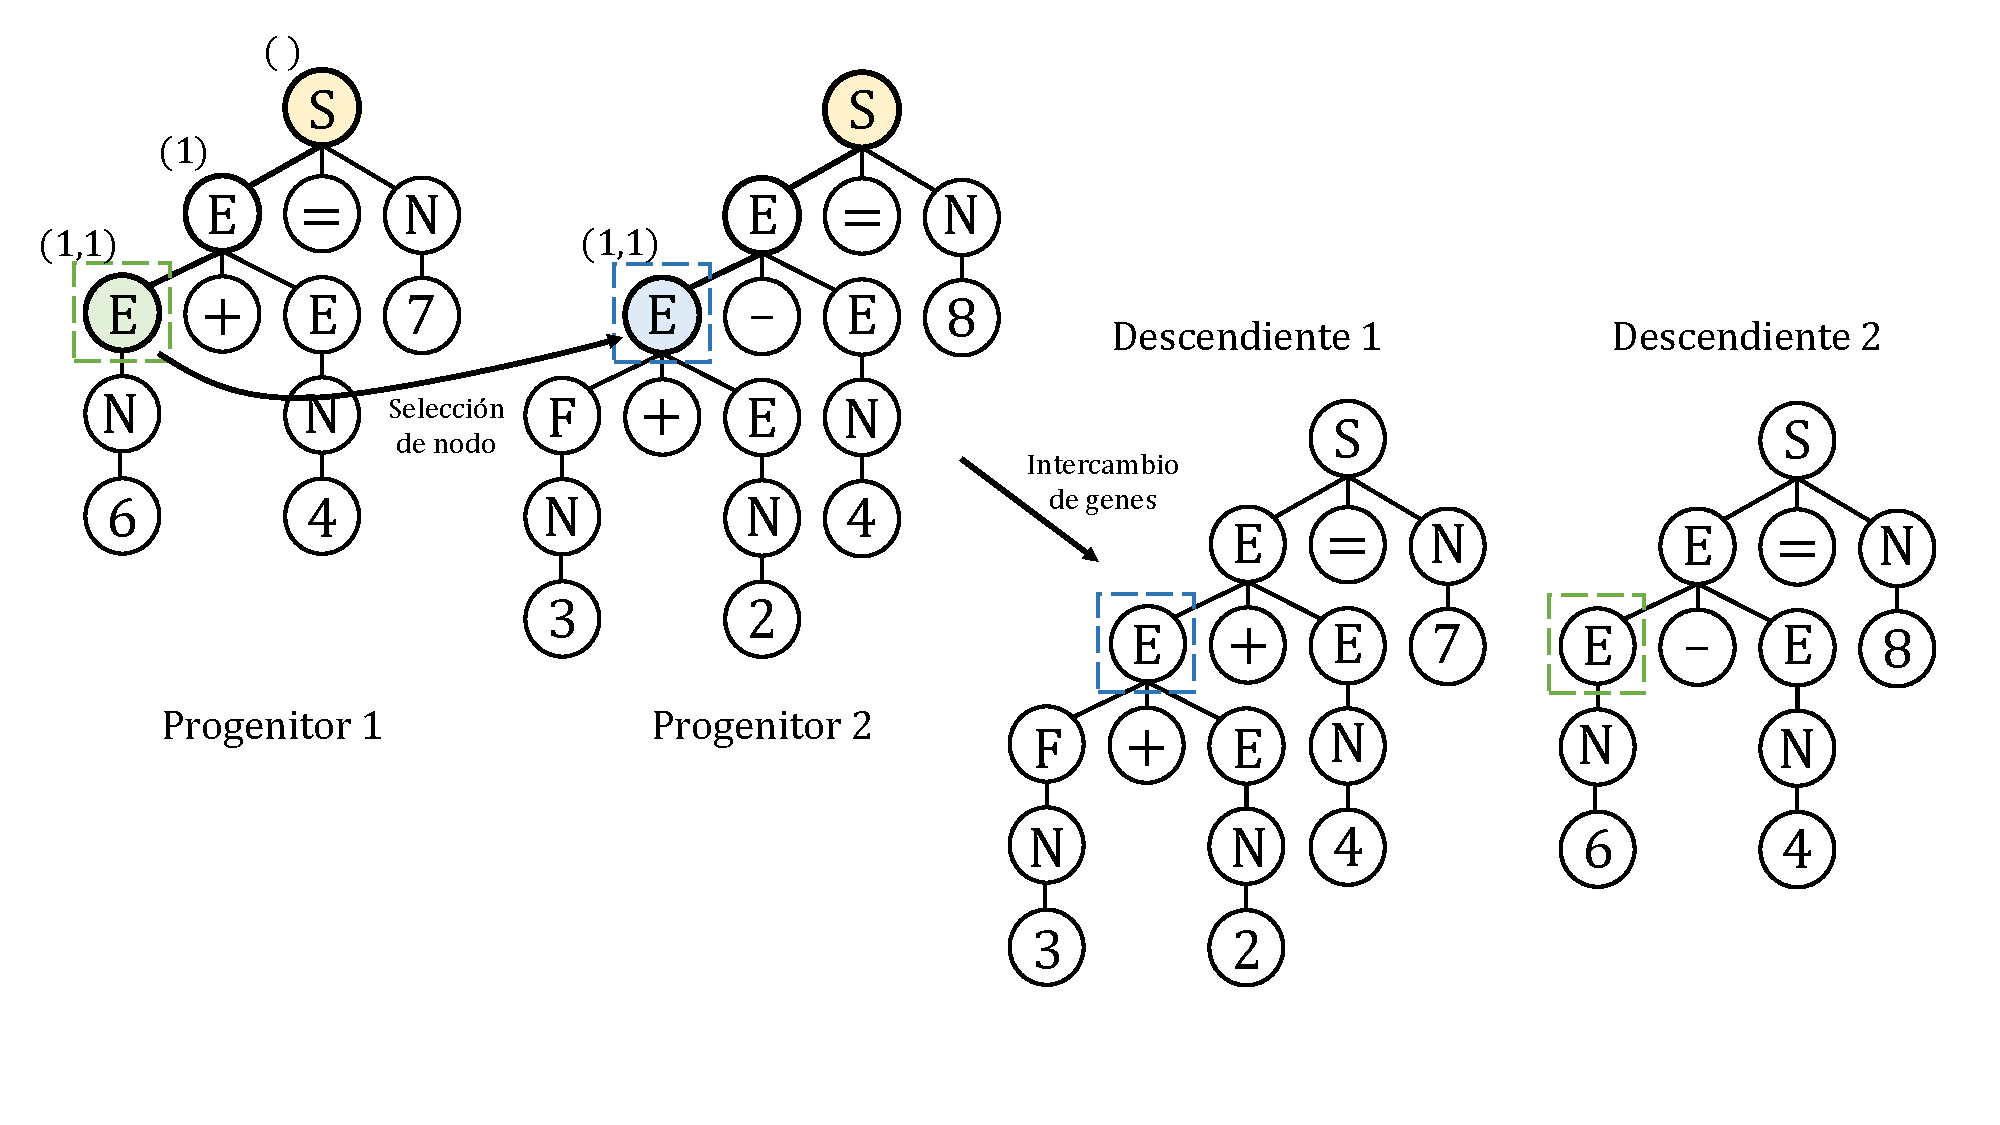
\includegraphics[width = 1\textwidth]{resources/Fig8.pdf}
          \caption{Ejemplo de aplicación del operador de cruce preservador del contexto.}
          \label{fig:8}
        \end{figure} \par
        El problema que tiene es que es útil para individuos que son estructuralmente similares, es decir, que habrá individuos que nunca se podrán cruzar, por lo que presenta serios problemas de exploración. Además, tiene amplia capacidad de explotación, por lo que, si bien es útil en fases tempranas del programa genético, produciría una convergencia demasiado rápida y problemas de caídas en óptimos locales. Tampoco limita la profundidad de los árboles, por lo que propicia la aparición de intrones.
        
        \subsubsection*{\vspace{-0.5cm}{\normalsize Operador de Whigham}}
        \vspace{-0.5cm}
        El operador de Whigham (Whigham, 1995) busca establecer un equilibrio entre exploración y explotación. No utiliza las coordenadas, sino que selecciona un símbolo no terminal (exceptuando el axioma) del primer progenitor, y, a continuación, de los símbolos no terminales del segundo progenitor, selecciona uno aleatorio de entre aquellos que son iguales al nodo del primer progenitor. En Fig. \ref{fig:9} se puede apreciar cómo funciona este operador. \par
        La única desventaja es que no controla la profundidad de los descendientes. Si se aplica sobre una gramática ambigua, puede generar individuos que representan la misma solución. Este operador también es utilizado en la Programación Genética tradicional, pero puede generar individuos no válidos, ya que en ella, todos los nodos interiores pueden ser elegidos. \par
        \begin{figure}[H]
          \centering
          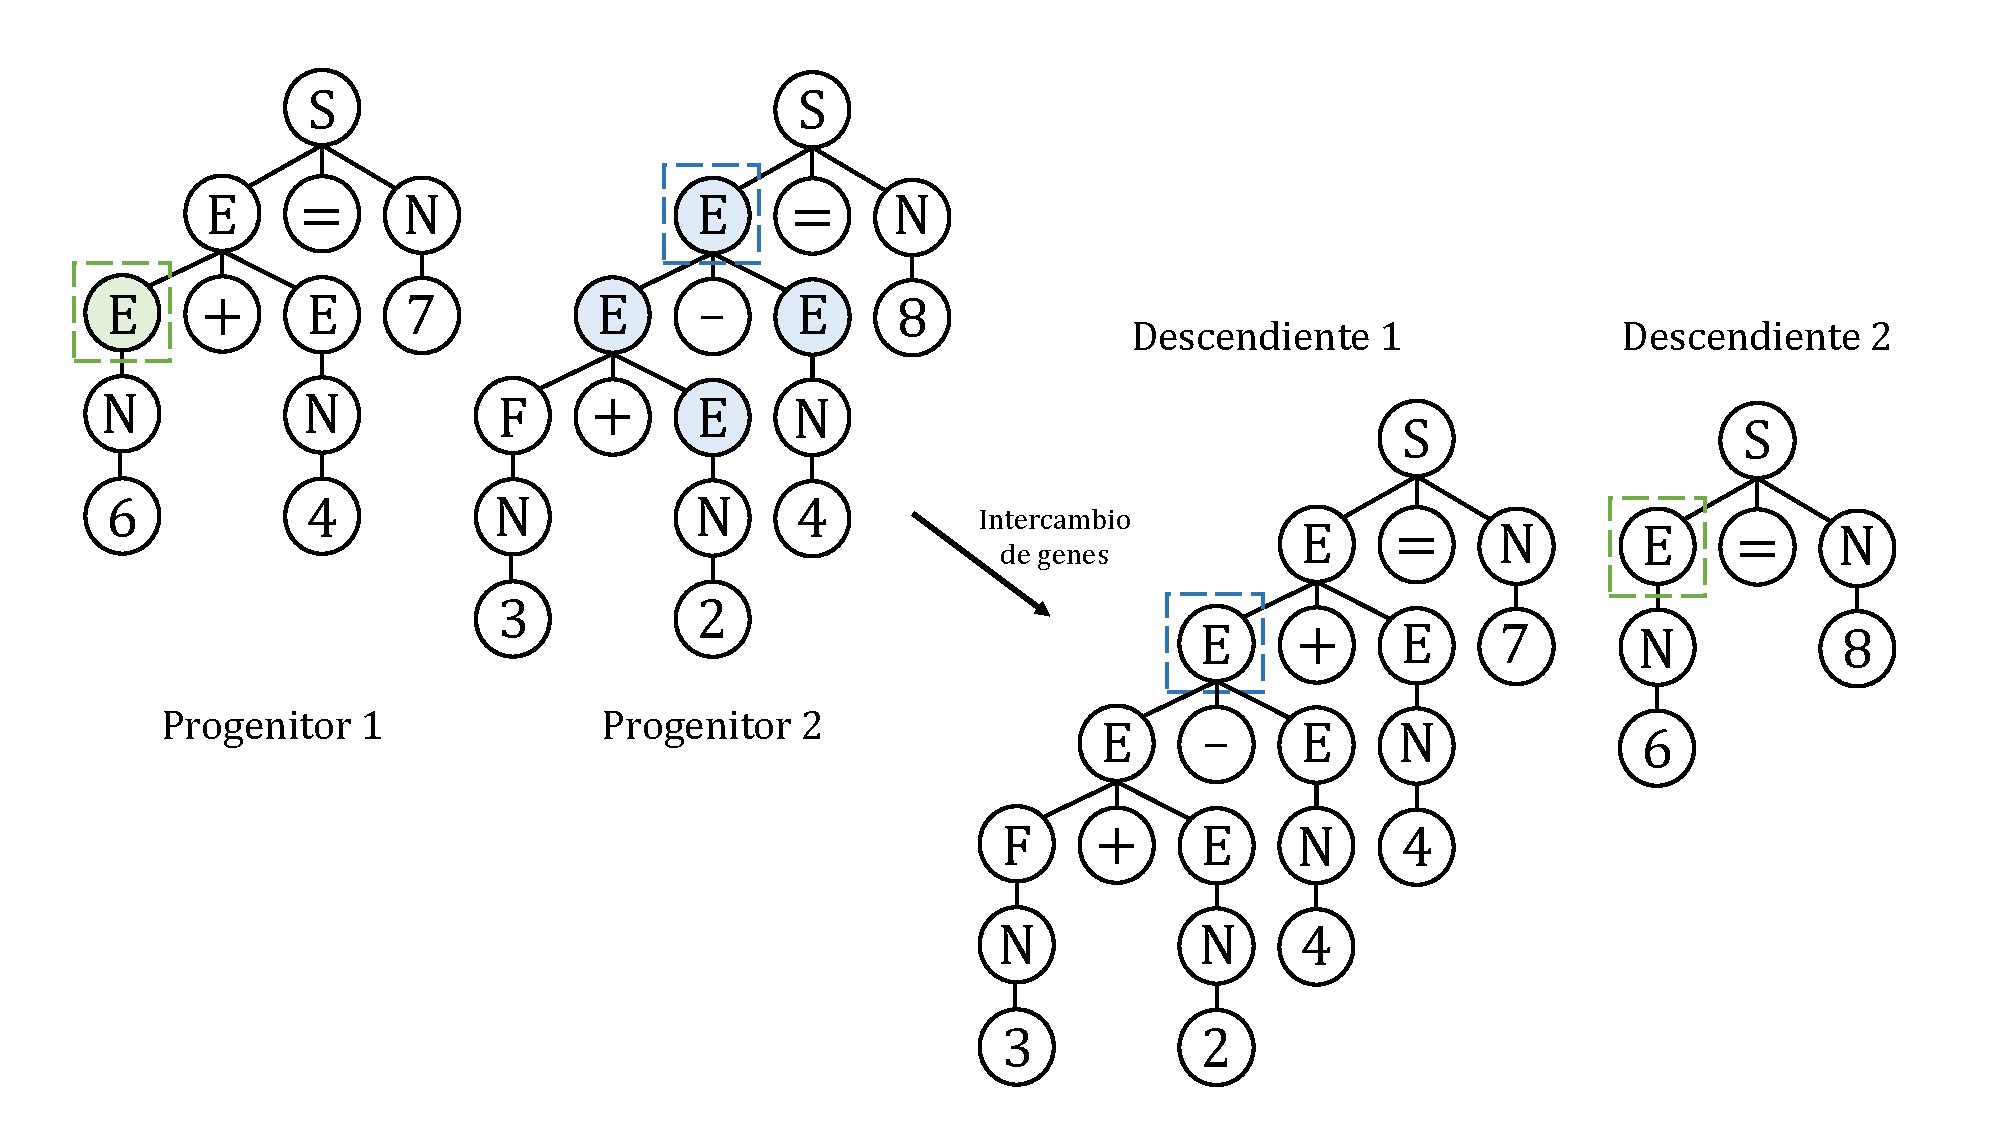
\includegraphics[width = 1\textwidth]{resources/Fig9.pdf}
          \caption{Ejemplo de aplicación del operador de cruce de Whigham.}
          \label{fig:9}
        \end{figure} \par
        
    \subsection*{\large 2.4.4. Generación de la población inicial}
    Para la creación de individuos para la población inicial, hay dos técnicas: una aleatoria y otra controlada. La primera de ellas, utiliza la Gramática Libre de Contexto y genera derivaciones de forma aleatoria, siguiendo las reglas de producción. A pesar de que genera individuos sintácticamente válidos y es simple de aplicar, además de óptimo en problemas de dominio reducido, es incapaz de controlar la profundidad, facilitando la aparición de la explosión de código. \par
    El segundo método es una variante del primero, ya que los individuos también se generan de forma aleatoria, pero controlando en todo momento la profundidad de la derivación, no permitiendo en ningún caso que se sobrepase la profundidad máxima. \vfill
    
  \chapter{\vspace{-3cm}{\LARGE 3. Redes de Neuronas Artificiales}}
  \setcounter{figure}{9}
  \vspace{-1cm}
  Las Redes de Neuronas Artificiales son un paradigma de procesamiento de información inspirado en cómo el sistema nervioso procesa la información. El sistema nervioso está compuesto por un gran número de unidades de procesamiento de información denominadas neuronas (\emph{neurons}) que trabajan al unísono para resolver problemas específicos. En este capítulo se ofrece, en primer lugar, un resumen de la \emph{historia} de las Redes de Neuronas Artificiales. Seguidamente, un apartado de \emph{funcionamiento general} sobre esta rama de estudio y que finaliza hablando de los distintos \emph{tipos} de redes.
  
    \section*{\Large 3.1. Historia}
    Los primeros trabajos sobre Redes de Neuronas Artificiales fueron los de McCulloch y Pitts (McCulloch and Pitts, 1943), que pronto se verían reforzados con las aportaciones de Hebb (Hebb, 1949) y Joseph Erlanger (1944), que aunque no tuvieran una aplicación directa sobre la Inteligencia Artificial, sus descubrimientos sobre el aprendizaje humano y las fibras de conexión entre neuronas, respectivamente, fueron clave en los siguientes años de desarrollo de las Redes de Neuronas Artificiales. Pocos años después aparece el primer desarrollo metodológico basado en Redes de Neuronas Artificiales: el Perceptrón (\emph{perceptron}) (Rosenblatt, 1958, 1962). \par
    Los años 60 fueron años de gran éxito en este ámbito. Destacó el trabajo de Widrow y Hoff (Widrow and Hoff, 1960): un sistema con un método de aprendizaje alternativo al Perceptrón llamado ADALINE (ADAptive LInear Element). Dos años después, estos científicos desarrollarían una mejora adaptativa sobre su sistema (Widrow and Hoff, 1962). Esta década finaliza con la publicación de un manual de referencia del Perceptrón por Minsky y Papert (Minsky and Papert, 1969), en el que además mostraban sus numerosos fallos y limitaciones como que no podía resolver el problema del XOR. \par
    A raíz de esta última publicación, el interés sobre el estudio de estos modelos de aprendizaje se perdió, hasta tal punto que pasarían más de 10 años hasta la aparición de nuevos trabajos. Este silencio sería roto por Klopf (Klopf, 1972), quien formuló un mecanismo de aprendizaje adaptativo. Dos años más tarde, se publica el famoso método de aprendizaje de propagación hacia atrás (\emph{back-propagation learning method}) (Werbos, 1974), que no sería verdaderamente apreciado hasta finales de los años 80. También, apareció la primera publicación sobre una red multicapa para interpretar caracteres manuscritos: las Redes de Neuronas Artificiales Convolucionales (Fukushima, 1975). Este trabajo consigue despertar el interés de algunos investigadores, pero sin mucho éxito. \par
    Los años 80 y 90 cerrarían esta historia, corta pero fructuosa sobre las Redes de Neuronas Artificiales, proganizados, en primer lugar, por la publicación del mapa (o red) de Kohonen (\emph{Kohonen map}) (Kohonen, 1982). En segundo lugar, se publicó una metodología sobre de Redes de Neuronas Artificiales Recurrentes (Hopfield, 1982), que tuvo un efecto contrario a la publicación de Minsky y Papert, persuadiendo a cientos de investigadores, que recobraron el interés en la investigación en este ámbito. Además, la tesis de Werbos vería en esta época su implicación gracias al trabajo de Rumelhart (Rumelhart et al., 1986), que propuso el método de aprendizaje del gradiente descendente (\emph{gradient descent learning method}).
    
    \section*{\Large 3.2. Funcionamiento general}
    Las Redes de Neuronas Artificiales son un modelo de procesamiento de información inspirado en cómo los sistemas nerviosos en la biología, como el cerebro, procesan información. En términos simples, una Red de Neuronas Artificiales es un modelo matemático del cerebro que es utilizado para procesar relaciones no lineales entre las entradas (\emph{inputs}) y las salidas (\emph{outputs}) en paralelo tal y como el cerebro humano hace todo el tiempo. \par
    En Fig. \ref{fig:10} se puede apreciar la arquitectura de un Perceptrón con una neurona artificial (o una red con una única neurona). Una neurona artificial recibirá un conjunto determinado de entradas (en este caso, $n$), con sus respectivos pesos sinápticos (\emph{synaptic weights}). A continuación, calculará el potencial sináptico (\emph{synaptic potential}) como la suma de los productos entre las entradas por sus respectivos pesos. A este potencial se le aplica una función de activación (\emph{activation function}), relativa a cada neurona, que permite devolver una salida $y$, en función del estado de activación. \par
    \begin{figure}[H]
      \centering
      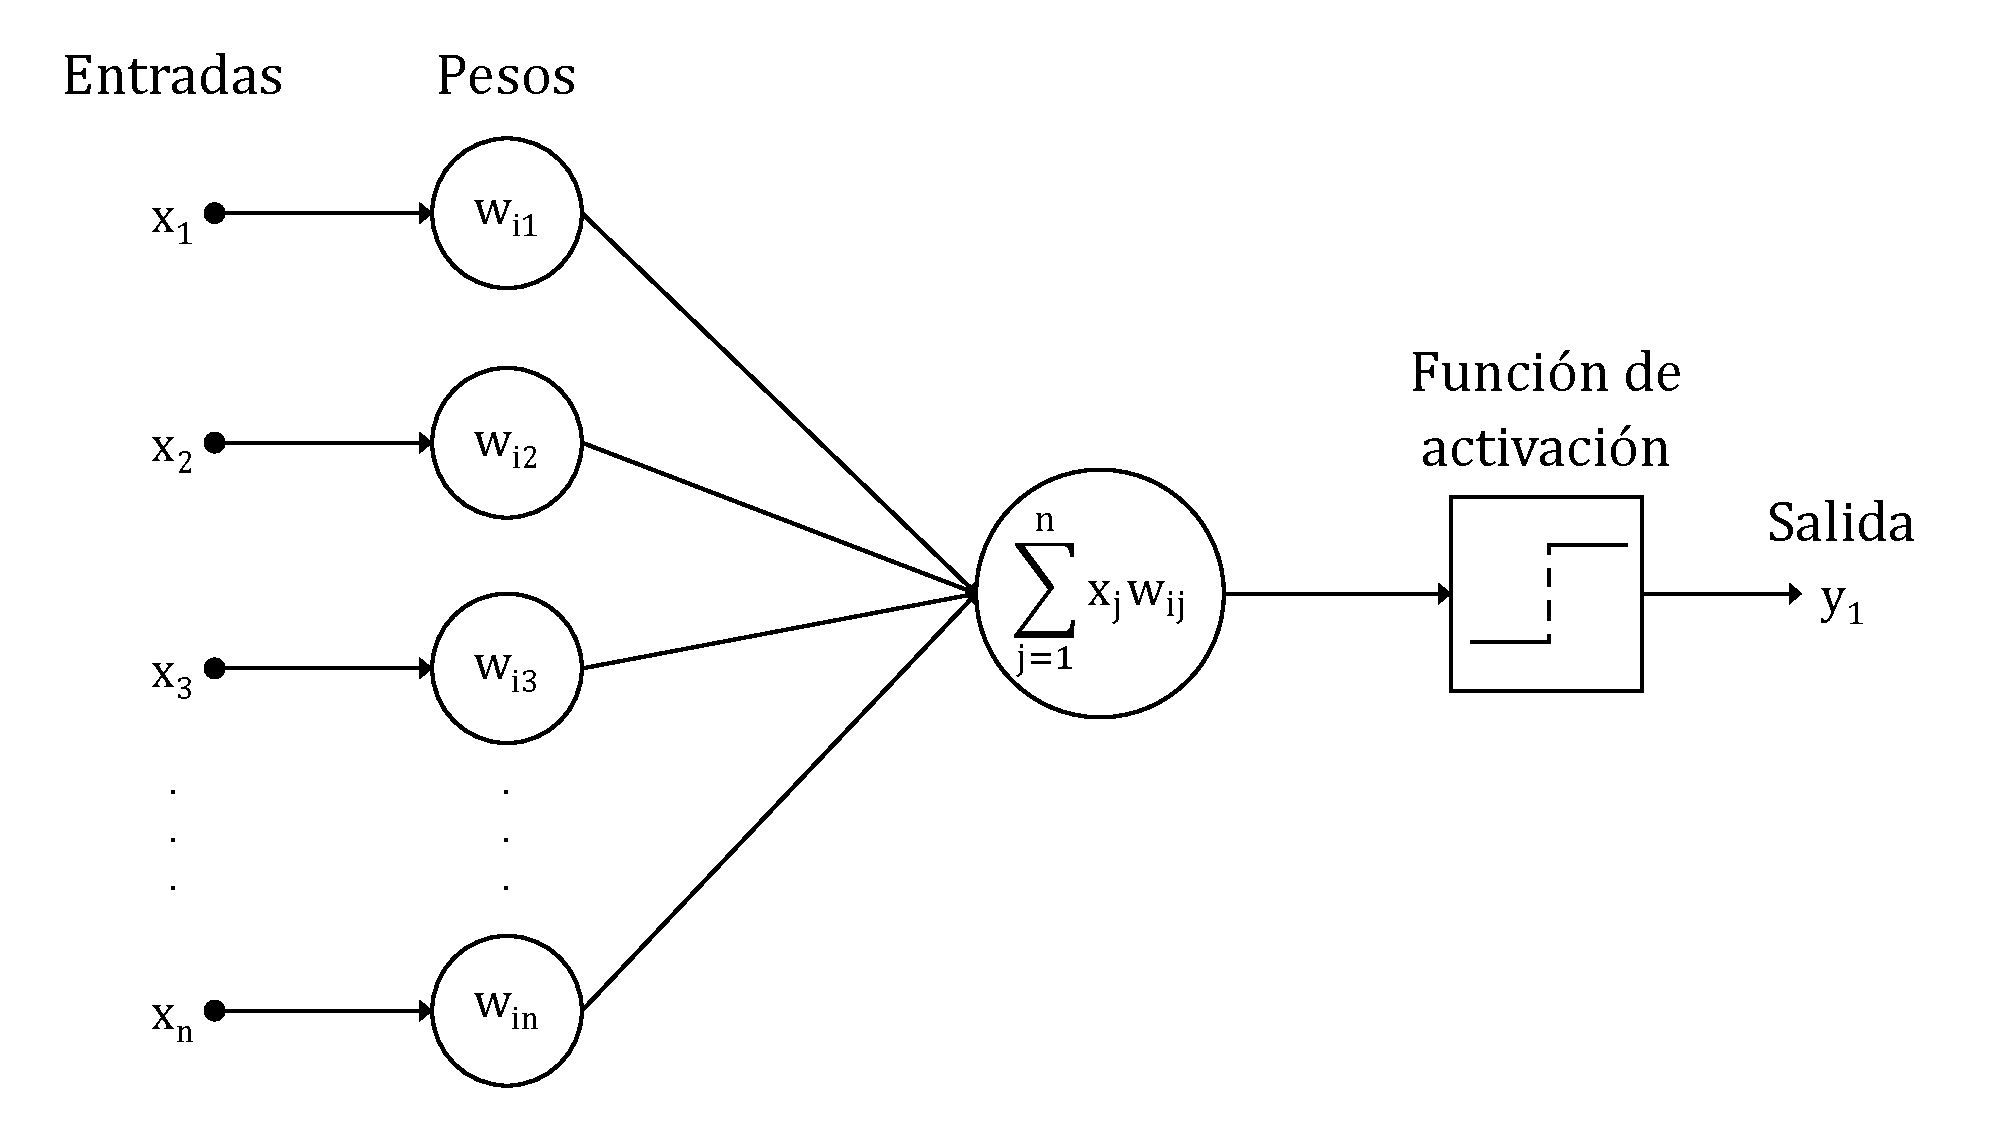
\includegraphics[width = 0.8\textwidth]{resources/Fig10.pdf}
      \caption{Arquitectura básica de un Perceptrón.}
      \label{fig:10}
    \end{figure} \par
    Sin embargo, la arquitectura de una red no es tan simple como la mostrada en Fig. \ref{fig:10}. Una Red de Neuronas Artificiales que no es un Perceptrón suele componerse por, al menos, una capa oculta (\emph{hidden layer}). Cuando una red tiene más de una capa oculta (es decir, más de 3 capas incluyendo la de entrada y la de salida), la red se denomina Red de Neuronas Artificiales Profunda (\emph{deep artificial neural network}) (Aizenberg et al., 2000). En Fig. 11 se muestra una arquitectura profunda con 2 capas ocultas. \par
    \begin{figure}[H]
      \centering
      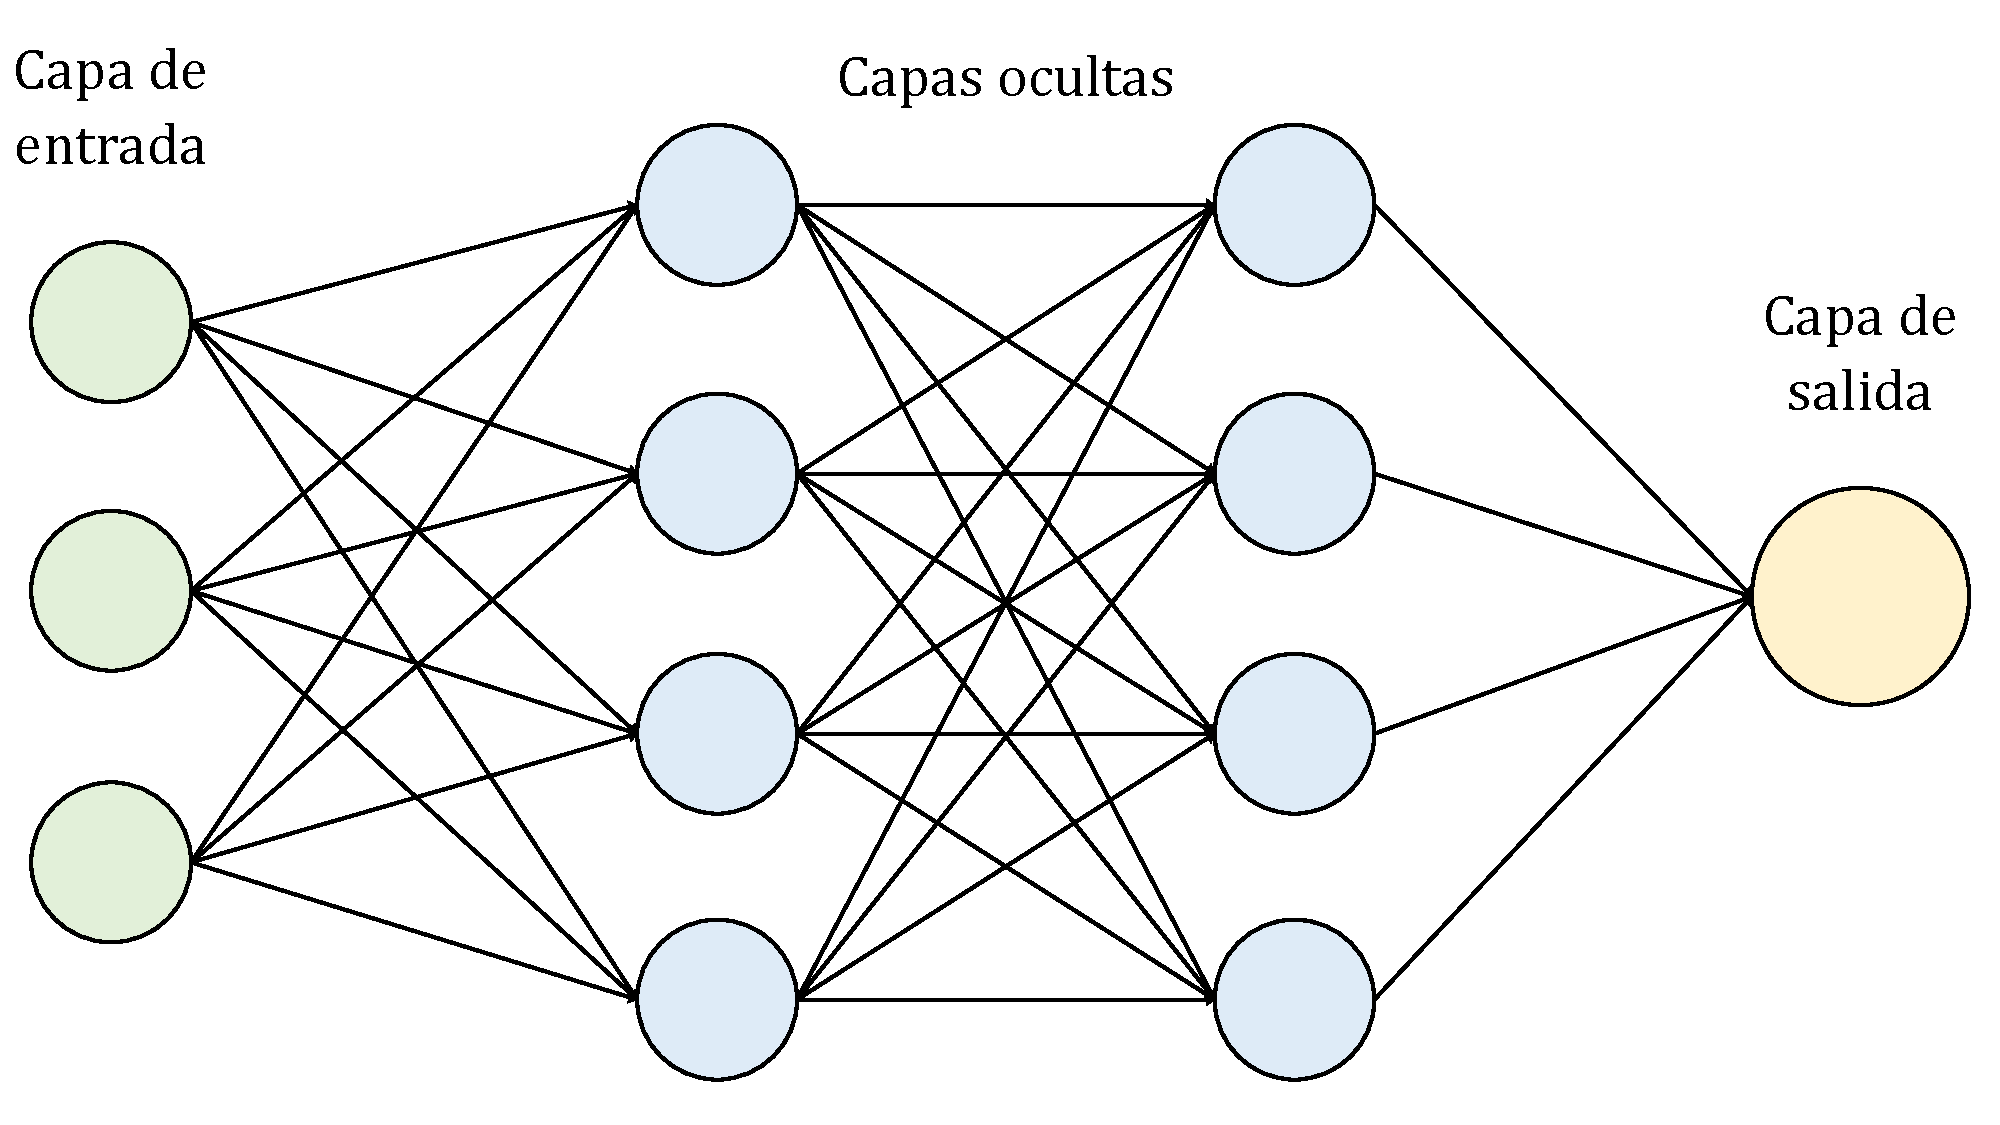
\includegraphics[width = 0.8\textwidth]{resources/Fig11.pdf}
      \caption{Distintas capas de una Red de Neuronas Artificiales.}
      \label{fig:11}
    \end{figure} \par
    En la capa de entrada (\emph{input layer}), las neuronas reciben datos o señales procedentes del entorno. Las neuronas de la capa de salida (\emph{output layer}) proporcionan la respuesta de la red a los estímulos de la entrada, aplicando una transformación que se lleva a cabo a lo ancho de la red. Entre la capa de entrada y la de salida están las capas ocultas (\emph{hidden layers}), que no reciben ni suministran informacion al entorno, sino que la modifican ya que llevan a cabo el procesamiento interno de la red. \par
    El proceso que sigue una Red de Neuronas Artificiales al actualizar los pesos se denomina aprendizaje y está determinado por el paradigma; si es o no un aprendizaje supervisado y por el algoritmo que utiliza para llevarlo a cabo. Con el aprendizaje supervisado, se supone que el usuario conoce la clasificación de aquello que desea clasificar, por lo que la red intentará minimizar el error entre la etiqueta que predice y su valor real para que la salida obtenida termine siendo la real. En cambio, en el aprendizaje no supervisado, la red recibe un conjunto de patrones de los que no conoce la respuesta deseada, e intentará extraer sus rasgos y agruparlos por similaridad. \par
    Cada neurona tiene asociada una función de activación. Existen muchas funciones, cada una con sus ventajas y desventajas, y adecuadas para ser utilizadas según ciertos criterios. Además, algunas de estas funciones tienen limitaciones, como la lineal, que no permite utilizar la propagación hacia atrás para entrenar el modelo, ya que su derivada es una constante y no tiene relación con la entrada. En Fig. 12 se muestran las funciones de activación más destacadas.
    %www.mini.pw.edu.pl/~macukow/wspolne/selection.pdf
    \begin{figure}[H]
      \begin{minipage}{0.5\textwidth}
        \centering
        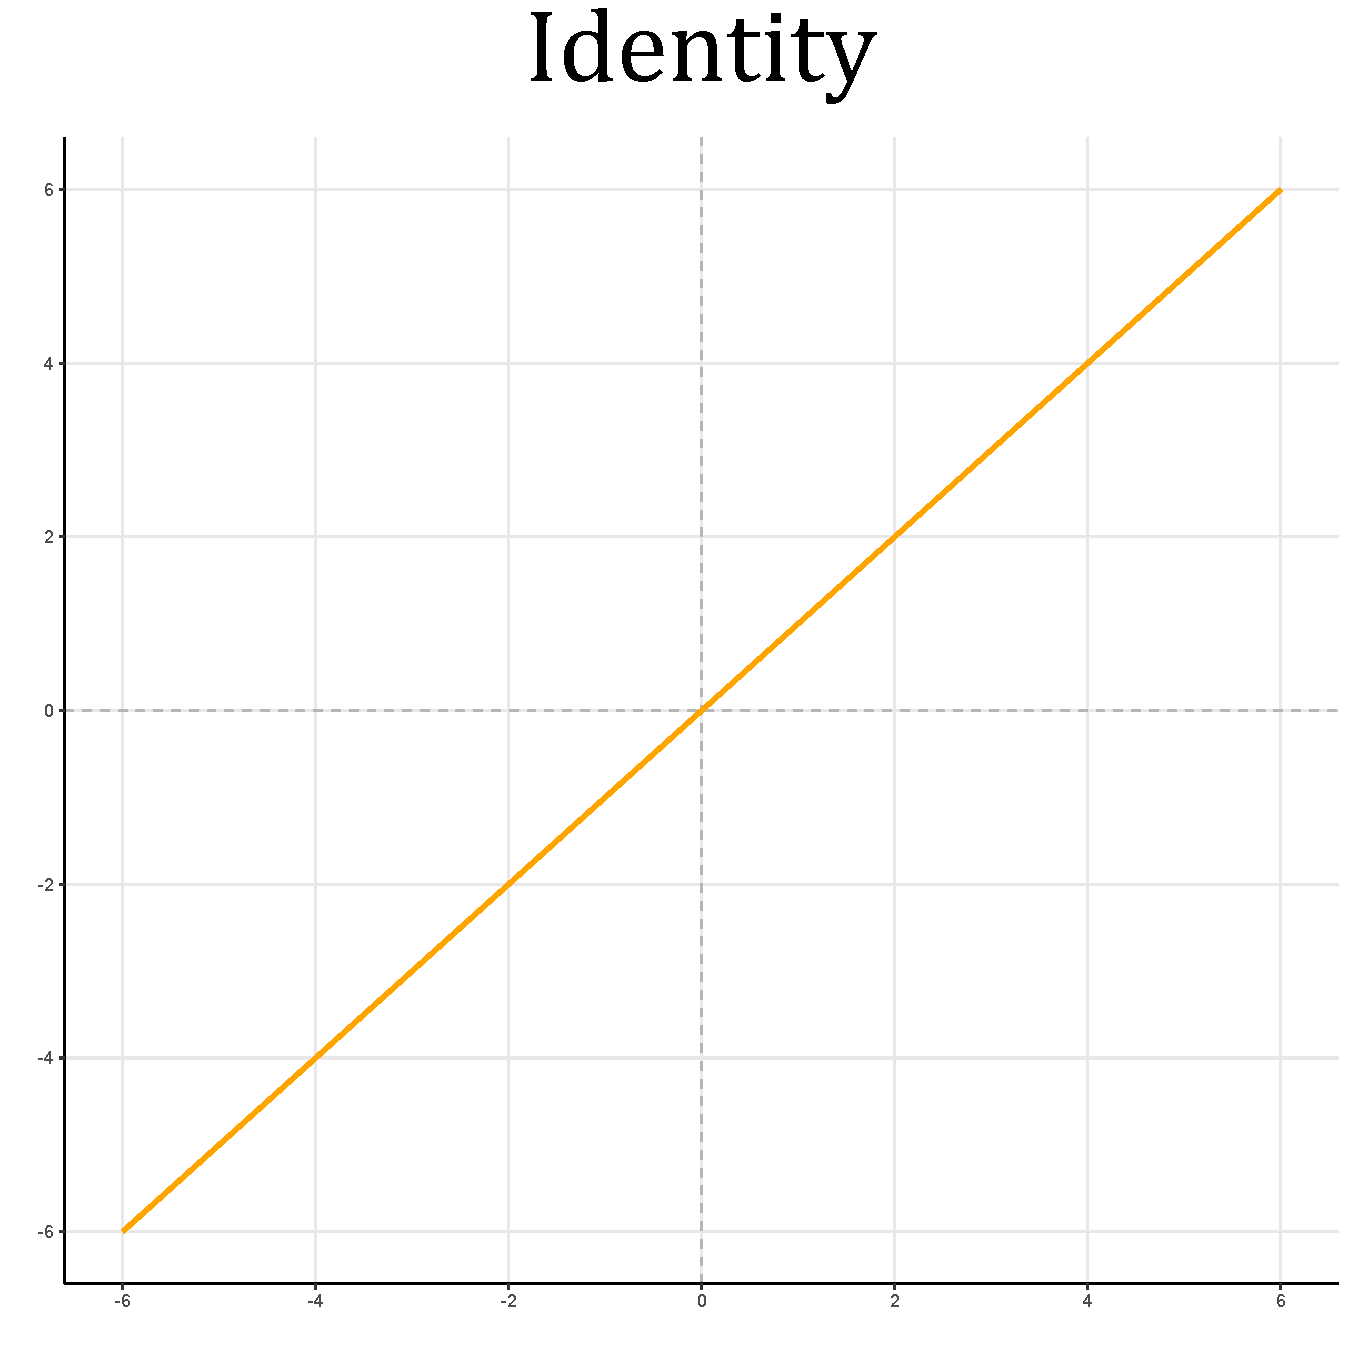
\includegraphics[width = 0.7\linewidth]{resources/Fig12_1.pdf}
      \end{minipage}l
      \begin{minipage}{0.49\textwidth}
        \centering
        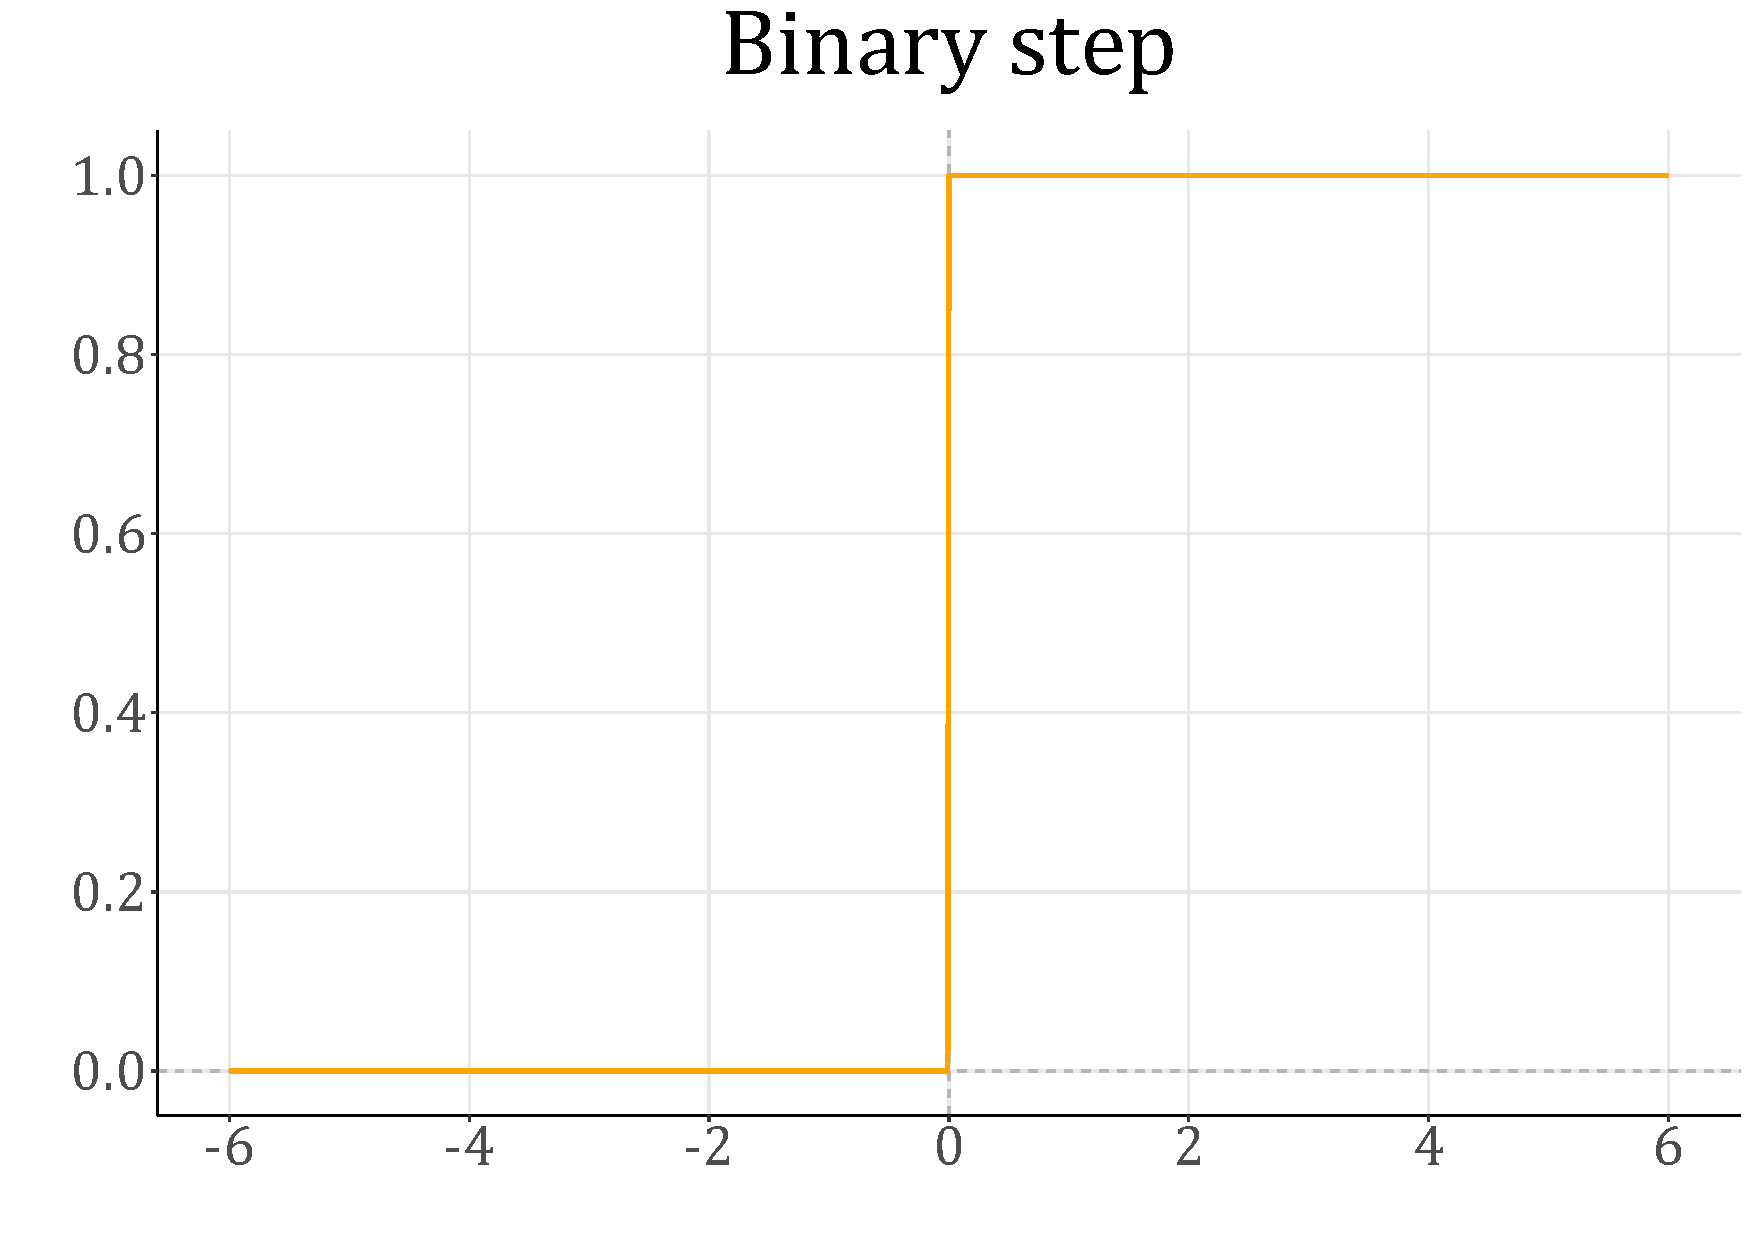
\includegraphics[width = 0.7\linewidth]{resources/Fig12_2.pdf}
      \end{minipage}
    \end{figure}
    \section*{\Large 3.3. Tipos}
    
  
  \chapter{\vspace{-3cm}{\LARGE 4. Construcción de Redes de Neuronas}}
  
  \chapter{\vspace{-3cm}{\LARGE 5. Planteamiento del problema}}
  
  \chapter{\vspace{-3cm}{\LARGE 6. Solución propuesta}}
  
  \chapter{\vspace{-3cm}{\LARGE 7. Resultados}}
  
  \chapter{\vspace{-3cm}{\LARGE 8. Conclusiones y líneas futuras}}
  \vfill
  
  \begin{thebibliography}{00}
  \vspace{-1cm}
  \makeatletter
  \def\@biblabel#1{}
  \let\old@bibitem\bibitem
  \def\bibitem#1{\old@bibitem{#1}\leavevmode\kern-\bibindent}
  \makeatother
  
  \bibitem{Aizenberg2000} Aizenberg, I., Aizenberg, N.N. and Vandewalle, J.P.L. (2000). \emph{Multi-Valued and Universal Binary Neurons: Theory, Learning and Applications}.
  \bibitem{Banzhaf1998} Banzhaf, W., Poli, R., Schoenauer, M. and Fogarty, T.C. (1998). \emph{Genetic Programming}.
  \bibitem{Beni1989} Beni, G. and Wang, J. (1989). Swarm intelligence in cellular robotic systems. \emph{Proceedings5 of the NATO Advance Workshop on Robots and Biological Systems}. 102:703-712.
  \bibitem{Beni2004} Beni, G. (2004). From Swarm Intelligence to Swarm Robotics. \emph{International Workshop on Swarm Robotics}. 3342:1-9.
  \bibitem{Boyd2004} Boyd, S. and Vandenberghe, L. (2004). Convex Optimization. \emph{Cambridge University Press 2004}: 129.
  \bibitem{Box1957} Box, G.E.P. (1957). Evolutionary operation: A method for increasing industrial productivity. \emph{Journal of the Royal Statistical Society. Series C}. 6(2):81-101.
  \bibitem{Box1969} Box, G.E.P. and Draper, N.P. (1969). \emph{Evolutionary Operation. A method for Increasing Industrial Productivity}.
  \bibitem{Bremermann1962} Bremermann, H.J. (1962). Optimization through evolution and recombination. \emph{Self-Organizing Systems 1962}: 93-106.
  \bibitem{Chomsky1959} Chomsky, N. (1959). On Certain Formal Properties of Grammars. \emph{Information and Control}. 2(2):137-167.
  \bibitem{Couchet2006} Couchet, J. and Manrique, D. (2006). Crossover and mutation operations for grammar-guided genetic programming. \emph{Soft Computing}. 11(10):943-955.
  \bibitem{Cramer1985} Cramer, N.L. (1985). A representation for the Adaptive Generation of Simple Sequential Programs. \emph{Proceedings of the First International Conference on Genetic Algorithms and the Applications}: 183-187.
  \bibitem{Dhaeseleer1994} D'haeseleer, P. (1994). Context preserving crossover in genetic programming. \emph{Proceedings of the First IEEE Conference on Evolutionary Computation}. 1:256-261.
  \bibitem{Dantzig1990} Dantzig, G.B. (1990). Origins of the simplex method. \emph{A history of scientific computing}, pages 141-151.
  \bibitem{Darwin1859} Darwin, C. (1859). \emph{On the Origin of Species by Means of Natural Selection, or Preservation of Favoured Races in the Struggle for Life}. 
  \bibitem{deAraujo2014} De Araujo, A.F. and Tavares, J.M.R.S. (2014). An Artificial Life Model for Image Enhancement. \emph{15th International Conference on Experimental Mechanics}. 41(13):5892-5906.
  \bibitem{Deb2002} Deb, K., Agarwal, S., Pratap, A. and Meyarivan, T. (2002). A Fast and Elitist Multiobjective Genetic Algorithm: NSGA-II. \emph{IEEE Transactions on Evolutionary Computation}. 6(2):128-197.
  \bibitem{Farmer1986} Farmer, J.D., Packard, N.H. and Perelson, A.S. (1986). The Immune System, Adaptation, and Machine Learning. \emph{Physica D: Nonlinear Phenomena}. 22(1): 187-204.
  \bibitem{Fogel1966} Fogel, L.J., Owens, A.J. and Walsh, M.J. (1966). \emph{Artificial Intelligence through Simulated Evolution}.
  \bibitem{Fraser1957} Fraser, A.S. (1957). Simulation of Genetic Systems by Automatic Digital Computers. \emph{Australian journal of biological sciences}. 10:484-499.
  \bibitem{Friedberg1958} Friedberg, R.M. (1958). A learning machine: part I. \emph{IBM Journal of Research and Development}. 2(1):2-13.
  \bibitem{Friedberg1959} Friedberg, R.M., Dunham, B. and North, J.H. (1959). A learning machine: part II. \emph{IBM Journal of Research and Development}. 3(3):282-287.
  \bibitem{Fukushima1975} Fukushima, K. (1975). Cognitron: A self-organizing multilayered neural network. \emph{Biological Cybernetics}. 20(3):121-136.
  \bibitem{Geem2001} Geem, Z.W., Kim, J.H. and Loganathan, G.V. (2001) A New Heuristic Optimization Algorithm: Harmony Search. \emph{Simulation}, 76(2):60-68.
  \bibitem{Goldberg1989} Goldberg, D.E. (1989). \emph{Genetic Algorithms in Search, Optimization \& Machine Learning}.
  \bibitem{Grefenstette1985} Grefenstette, J.J. (1985). \emph{Proceedings of the First International Conference on Genetic Algorithms and the Applications} (Hillsdale, NJ: Lawrence Erlbaum).
  \bibitem{Grefenstette1987} Grefenstette, J.J. (1987). \emph{Proceedings of the Second International Conference on Genetic Algorithms and the Applications} (Hillsdale, NJ: Lawrence Erlbaum).
  \bibitem{Hassan2005} Hassan, R., Cohanim, B., de Weck, O. and Venter, G. (2005). A comparison of particle swarm optimization and the genetic algorithm. \emph{46th AIAA/ASME/ASCE/AHS/ASC Structures, Structural Dynamics and Materials Conference}.
  \bibitem{Hebb1949} Hebb, D.O. (1949). \emph{The Organization of Behavior}. (New York: Wiley).
  \bibitem{Holland1962} Holland, J.H. (1962). Nonlinear environments permitting efficient adaptation. \emph{Computer and Information Sciences II}: 147-164.
  \bibitem{Hopcroft1979} Hopcroft, J.E. and Ullman, J.D. (1979). Context-Free Grammars. \emph{Introduction to Automata Theory Languages and Computation}: 77-106.
  \bibitem{Hopfield1982} Hopfield, J.J. (1982). Neural networks and physical systems with emergent collective computational abilities. \emph{Proceedings of the National Academy of Sciences of the United States of America}. 79(8):2554-2558.
  \bibitem{Hu2014} Hu, T., Banzhaf, W. and Moore, J.H. (2014). The effects of recombination of phenotypic exploration and robustness in evolution. \emph{Artificial Life}. 20(4):457-470.
  \bibitem{Klopf1972} Klopf, A.H. (1972). Brain Function and Adaptive Systems - A Heterostatic Theory. \emph{Air Force Cambridge Research Laboratories}.
  \bibitem{Kohonen1982} Kohonen, T. (1982). Self-Organized Formation of Topologically Correct Feature Maps. \emph{Biological Cybernetics}. 43:59-69.
  \bibitem{Koza1988} Koza, J.R. (1988). Non-Linear Genetic Algorithms for Solving Problems. \emph{University States Patent 4935877}.
  \bibitem{Koza1992} Koza, J.R.(1992). \emph{Genetic Programming: On the Programming of Computers by Means of Natural Selection}  (Cambridge, MA: MIT Press).
  \bibitem{Koza1996} Koza, J.R., Goldberg, D.E., Fogel, D.B. and Riolo, R.L. (1996). \emph{Genetic Programming 1996} (Cambridge, MA: MIT Press).
  \bibitem{Kosorukoff2001} Kosorukoff, A. (2001). Human based genetic algorithm. \emph{2001 IEEE International Conference on Systems, Man and Cybernetics. e-Systems and e-Man for Cybernetics in Cyberspace}: 3464-3469.
  \bibitem{Langton1986} Langton, C.G. (1986). Studying artificial life with cellular automata. \emph{Physica D: Nonlinear Phenomena}. 22(1):120-149.
  \bibitem{McCulloch1943} McCulloch, W.S. and Pitts, W.H. (1943) A Logical Calculus of the Ideas Immanent in Nervous Activity. \emph{Bulletin of Mathematical Biophysics}. 5:115-133.
  \bibitem{Minsky1969} Minsky, M.L. and Papert, S. (1969). \emph{Perceptrons: An Introduction to Computational Geometry} (Cambridge: MIT Press).
  \bibitem{Moscato1989} Moscato, P. (1989). On Evolution, Search, Optimization, Genetic Algorithms and Martial Arts - Towards Memetic Algorithms. \emph{Caltech Concurrent Computation Program}: 158-179.
  \bibitem{Nocedal1999} Nocedal, J. and Wright, S.J. (1999). Numerical optimization. \emph{Springer-Verlag}.
  \bibitem{Pezzella2008} Pezzella, F., Morganti, G. and Ciaschetti, G. (2008). A genetic algorithm for the Flexible Job-shop Scheduling Problem. \emph{Computers \& Operations Research}. 35(10):3202-3212.
  \bibitem{Poli1997a} Poli, R. and Langdon, W.B. (1997a). An experimental analysis of schema creation, propagation and disruption in genetic programming. \emph{Proc. of ICGA'97}.
  \bibitem{Poli1997b} Poli, R. and Langdon, W.B. (1997b). A new schema theory for genetic programming with one-point crossover and point mutation. \emph{Proc. of the Second On-line World Conference on Soft Computing in Engineering Design and Manufacturing}.
  \bibitem{Poli1998} Poli, R. and Langdon, W.B. (1998). A review of theoretical and experimental results on schemata in genetic programming. \emph{Proceedings of the First European Workshop on Genetic Programming}.
  \bibitem{Polya1945} Polya, G. (1945). How to Solve It. \emph{Princeton University Press 1945}.
  \bibitem{Rawlins1991} Rawlins, G.J.E. (1991). \emph{Foundations of Genetic Algorithms} (San Mateo, CA: Morgan Kaufmann).
  \bibitem{Rechenberg1965} Rechenberg, I. (1965). Cybernetic Solution Path of an Experimental Problem. \emph{Royal Aircraft Establishment Library Translation 1122}.
  \bibitem{Reynolds1994} Reynolds, R.G. (1994). An Introduction to Cultural Algorithms. \emph{Proceedings of the 3rd Annual Conference on Evolutionary Programming}: 131-139.
  \bibitem{Roberts1965} Roberts, L. (1965). Machine perception of 3D solids. \emph{Optical and Electro-Optical Information Processing}. 9:159-197.
  \bibitem{Rosenblatt1958} Rosenblatt, F. (1958). The Perceptron: A Probabilistic Model for Information Storage and Organization in The Brain. \emph{Psychological Review}. 65(6):386-408.
  \bibitem{Rosenblatt1962} Rosenblatt, F. (1962). \emph{Principles of Neurodynamics} (Washington: Spartan Books). 
  \bibitem{Rumelhart1986} Rumelhart, D.E., Hinton, G.E. and Williams, R.J. (1986). Learning internal representations by error propagation. \emph{Parallel Distributed Processing: Explorations in the Microstructure of Cognition}. 1:318-362.
  \bibitem{Ryan1998} Ryan, C., Collins, J.J. and O'Neil, M. (1998). Grammatical Evolution: Evolving Programs for an Arbitrary Language. \emph{Proceedings of the First European Workshop on Genetic Programming}: 83-96.
  \bibitem{Samuel1959} Samuel, A.L. (1959). Some Studies in Machine Learning Using the Game of Checkers. \emph{IBM Journal of Research and Development}. 3(3):210-229.
  \bibitem{Schaffer1989} Schaffer, J.D. (1989). \emph{Proceedings of the Third International Conference on Genetic Algoritms and the Applications} (San Mateo, CA: Morgan Kaufmann).
  \bibitem{Schwefel1965} Schwefel, H-P. (1965). Kybernetische Evolution als Strategie der experimentellen Forschung in der Strömungstechnik.
  \bibitem{Storn1996} Storn, R. (1996). On the usage of differential evolution for function optimization. \emph{Biennial Conference of the North American Fuzzy Information Processing Society}: 519-523.
  \bibitem{Storn1997} Storn, R. and Price, K. (1997). Differential evolution - a simple and efficient heuristic for global optimization over continuous spaces. \emph{Journal of Global Optimization}. 11(4):341-359.
  \bibitem{Tackett1995} Tackett, W.A. (1995). Greedy Recombination and Genetic Search on the Space of Computer Programs. \emph{Foundations of Genetic Algorithms III} (San Mateo, CA: Morgan Kaufmann).
  \bibitem{Vanneschi2010} Vanneschi, L., Gustafson, S. and Banzhaf, W. (2010). Open issues in Genetic programming. \emph{Genetic Programming and Evolvable Machines}. 11:339-363.
  \bibitem{Vose1995} Vose, M.D. and Whitley, L.D. (1995). \emph{Foundations of Genetic Algorithms 3} (San Francisco, CA: Morgan Kaufmann).
  \bibitem{Waibel1989} Waibel, A., Hanazawa, T., Hinton, G., Shikano, K. and Lang, K.J. (1989). Phoneme recognition using time-delay neural networks. \emph{IEEE Transactions on Acoustics, Speech, and Signal Processing}. 37(3):328-339.
  \bibitem{Werbos1974} Werbos, P. (1974). \emph{Beyond regression: New tools for predicting and analysis in the behavioral sciences} (Doctoral dissertation).
  \bibitem{Whigham1995} Whigham, P.A. (1995). Grammatically-based genetic programming. \emph{Proceedings of the workshop on genetic programming: from theory to real-world applications}: 33-41.
  \bibitem{Whitley1993} Whitley, L.D. (1993). \emph{Foundations of Genetic Algorithms 2} (San Mateo, CA: Morgan Kaufmann).
  \bibitem{Widrow1960} Widrow, B. and Hoff, M. (1960). Adaptive Switching Circuits. \emph{International Journal of Communications, Network and System Sciences}. 5:96-104.
  \bibitem{Widrow1962} Widrow, B. and Hoff, M. (1962). Associative Storage and Retrieval of Digital Information in Networks of Adaptive “Neurons”. \emph{Biological Prototypes and Synthetic Systems}. 1:160-160.
  \end{thebibliography}
  
\end{document}
